\section{Mode Collapse and Verified Replay}
\label{app:theory}

We separate the per-prompt mean gradient from the geometry and noise of its
updates. Outcome-binary score estimators share a correctness-gradient
direction for differentiable neural policies, while their covariance can
differ. The categorical specialization yields finite-step concentration and
sampled symmetry breaking; fixed-bank replay has an explicit restoration
threshold and recovery bound. Complete-response and local-update arguments
state conditions for neural retention. We apply established replicator,
policy-gradient, information-theoretic, and coverage results where their
assumptions match: the sharpened replay certificate follows by KL data
processing, and exact Dr.GRPO with reference KL inherits a published
convergence guarantee. Our derivations address the group estimators, their
sampling noise, and the competition with the verified bank. These results
do not certify the implemented AdamW/PPO trajectories.
Table~\ref{tab:notation} lists the symbols used here.

\subsection{Categorical abstraction and mean updates}
\label{app:theory-grpo-mean}

The categorical results use the following model. The neural score identities,
finite-step updates, and sampled-update results below state separately which
assumptions they replace; none identifies a neural mode with an independently
optimized logit.

\begin{assumption}[Categorical mean-flow model]
\label{ass:categorical-mean-flow}
Fix one isolated prompt and a finite category set
$\mathcal A=\mathcal C\mathbin{\dot\cup}\mathcal N$ with $m\ge2$ correct
execution modes and $n\ge1$ incorrect categories, and set
$p_a=\operatorname{softmax}(z)_a$, $P=\sum_{c\in\mathcal C}p_c$, and
$q_c=p_c/P$, so that $P$ measures correctness while $q$ describes how that
correct probability is allocated among the individual correct modes.
\begin{enumerate}
\item[(A1)] \emph{Independent logits.} The policy carries one independently
  optimized logit for every category in $\mathcal A$, including one separate
  logit for each canonical correct mode.
\item[(A2)] \emph{Common length normalization.} Every response shares a single
  length scale, which is absorbed into the positive coefficient of the group
  estimator, rather than a scale that varies from one response to the next
  within the same rollout group.
\item[(A3)] \emph{Euclidean mean flow.} Updates are the infinitesimal expected
  updates in these logits, taken without optimizer preconditioning and without
  momentum carried between steps.
\item[(A4)] \emph{No competing regularizer.} Explicit reference KL is zero and
  no entropy term is present.
\item[(A5)] \emph{Nondegenerate start.} Logits are finite initially,
  $0<P(0)<1$, and the group size is $G\ge2$.
\end{enumerate}
\end{assumption}

We write ``under Assumption~\ref{ass:categorical-mean-flow}'' for (A1)--(A5)
together. Each limitation of the analysis can be traced to a specific item:
AdamW and PPO violate (A3), variable-length GRPO violates (A2), and entropy
regularization violates (A4).

A language model induces probabilities over canonical outcomes, but this
identification of probabilities does not identify its update geometry.
Aggregating several response strings into a mode does not generally commute
with gradient flow in response logits. One independent logit per canonical
outcome is therefore an explicit abstraction, not a reduction proved for the
neural policy or its validator equivalence classes.

Draw a group $Z_1,\ldots,Z_G\stackrel{\mathrm{iid}}{\sim}p$ with $G\ge2$,
write $R_i=\1[Z_i\in\mathcal C]$, and let $R=\sum_iR_i$. At the on-policy
point where the PPO ratio equals one, consider the common-length estimator
\begin{equation}
  \widehat g_G
  =\frac1G\sum_{i=1}^G
   w(R)\left(R_i-\frac{R}{G}\right)\nabla_z\log p_{Z_i}.
  \label{eq:group-estimator}
\end{equation}
For the Dr.GRPO abstraction, $w(R)=1$ after absorbing the shared positive
length scale. Reward-standardized GRPO with equal or common response-length
normalization takes $w(R)$ to be the reciprocal group reward standard
deviation on mixed groups (with a fixed numerical stabilizer if used).
Standard variable-length GRPO also weights each response by its own inverse
length \citep{shao2024deepseekmath,liu2025understanding}; that factor cannot
generally be absorbed into $w(R)$ and is outside the equivalence proved here.
In either included case, $0<w(\ell)<\infty$ for
$\ell\in\{1,\ldots,G-1\}$. We define the entire update as zero on all-equal
groups without evaluating an undefined reciprocal standard deviation;
likewise, $w(R)R(G-R)$ below is defined as zero when $R=0$ or $R=G$. All
advantages and normalization weights are detached in the score estimator.

\begin{lemma}[A group baseline does not remove frequency amplification]
\enforcehalffinalproseline
\label{lem:grpo-mean}
For $0<P<1$, the expected update in Equation~\eqref{eq:group-estimator} is
\begin{equation}
  \E[\widehat g_G]
  =c_G(P)\nabla_z P,
  \qquad
  c_G(P)=
  \frac{\E\!\big[w(R)R(G-R)\big]}{G^2P(1-P)}>0.
  \label{eq:expected-group-gradient}
\end{equation}
For the Dr.GRPO abstraction, $c_G(P)=(G-1)/G$. Group centering and reward
standardization rescale the expected gradient without changing its direction
under these assumptions.
\end{lemma}

\begin{proof}
\enforcehalffinalproseline
Condition on the complete binary reward vector, whose sum is $R$. The score
identities give
\[
  \E[\nabla_z\log p_{Z_i}\mid R_i=1]=\nabla_z\log P,
  \qquad
  \E[\nabla_z\log p_{Z_i}\mid R_i=0]
  =\nabla_z\log(1-P).
\]
There are $R$ correct rows with centered reward $(G-R)/G$ and $G-R$
incorrect rows with centered reward $-R/G$. Therefore the conditional
expectation of the unaveraged sum in~\eqref{eq:group-estimator} is
\[
  w(R)\frac{R(G-R)}{G}
  \left(\nabla_z\log P-\nabla_z\log(1-P)\right)
  =w(R)\frac{R(G-R)}{GP(1-P)}\nabla_zP.
\]
The outer factor $1/G$ and expectation over
$R\sim\operatorname{Binomial}(G,P)$ yield~\eqref{eq:expected-group-gradient}.
For $w\equiv1$,
$\E[R(G-R)]=G(G-1)P(1-P)$, proving the Dr.GRPO value.
\end{proof}

The binomial identity also gives the denominator-free expression
\[
 c_G(P)=\frac{G-1}{G}\sum_{j=0}^{G-2}\binom{G-2}{j}
 w(j+1)P^j(1-P)^{G-2-j}.
\]
The binomial weights sum to one, so $c_G$ lies between
$(G-1)\min_j w(j+1)/G$ and $(G-1)\max_j w(j+1)/G$.
This establishes the smooth, positive extension to $P=0,1$ used in the
subsequent flow and convergence arguments.

The next lemma specializes the practical-estimator analysis of
\citet[Section~4.3 and App.~D, Theorem~5]{tajwar2026maxrl}
to our categorical notation. We invoke that result directly and retain the
normalization that identifies the implemented estimator.

\begin{lemma}[Binary MaxRL has the same correctness-gradient direction]
\enforcehalffinalproseline
\label{lem:maxrl-mean}
Under Assumption~\ref{ass:categorical-mean-flow}, let MaxRL assign
$A_i^{\mathrm{MaxRL}}=GR_i/R-1$ when $R>0$ and zero when $R=0$, as in
Section~\ref{sec:method}. For
$\widehat g_G^{\mathrm{MaxRL}}=G^{-1}\sum_i
 A_i^{\mathrm{MaxRL}}\nabla_z\log p_{Z_i}$ at the on-policy point, the
expected update is
\begin{equation}
  \E[\widehat g_G^{\mathrm{MaxRL}}]
  =c_G^{\mathrm{MaxRL}}(P)\nabla_zP,
  \qquad
  c_G^{\mathrm{MaxRL}}(P)
  =\frac{1-(1-P)^{G-1}}{P}>0,
  \label{eq:maxrl-expected-gradient}
\end{equation}
with continuous endpoint values
$c_G^{\mathrm{MaxRL}}(0)=G-1$ and
$c_G^{\mathrm{MaxRL}}(1)=1$.
\end{lemma}

\begin{proof}
\enforcehalffinalproseline
Apply \citet[Theorem~5]{tajwar2026maxrl} with $N=G$ and pass rate $P$.
Its dropped-baseline estimator is exactly $\widehat g_G^{\mathrm{MaxRL}}$,
so its expected coefficient is $\sum_{j=0}^{G-2}(1-P)^j$.
The finite geometric sum gives Equation~\eqref{eq:maxrl-expected-gradient}
and its endpoint values. This application uses on-policy independent draws
and the score identity, without making an optimizer convergence claim.
\end{proof}

The same finite-series identity gives the potential used below:
\begin{equation}
 \Psi_{\mathrm{MaxRL}}(P)
 :=\int_0^P c_G^{\mathrm{MaxRL}}(s)\,ds
 =\sum_{k=1}^{G-1}\frac{1-(1-P)^k}{k}.
 \label{eq:maxrl-potential-finite-sum}
\end{equation}
In particular, $\Psi_{\mathrm{MaxRL}}(1)=\sum_{k=1}^{G-1}1/k$.
For binary rewards, best@\(k\) equals pass@\(k\), so this is a harmonic
mixture of sampling objectives for $k=1,\ldots,G-1$. The upper limit is
$G-1$, not $G$: the implemented centered estimator drops the entire update
on all-failure groups. Subtracting an unconditional score baseline even on
those groups instead gives the order-$G$ estimator. This distinction concerns
the exact finite-group expectation at the on-policy point; it does not assert
unbiasedness of subsequent clipped or adaptive-optimizer updates.


\subsection{Winner-take-all collapse in the categorical mean flow}
\label{app:theory-collapse}

Consider $\dot z=c_G(P)\nabla_zP$, with any of the smooth positive
coefficients established above: Dr.GRPO, common-length reward-standardized
GRPO, or the specified centered binary MaxRL estimator. This infinitesimal
expected-update model removes
sampling noise and retains independently trained Euclidean logits. The
conditional dynamics reduce to the standard frequency-dependent replicator
system with fitness $f_c(q)=q_c$
\citep{hofbauer1998evolutionary,harper2009informationgeometry}. The result is
a specialization to the group estimators, not a new general theorem about
replicator dynamics. Related correctness-indifferent collapse analyses include
\citet{sinha2026expected,lochab2026ucpo}.

\begin{theorem}[Standard replicator specialization for binary-reward RL]
\enforcehalffinalproseline
\label{thm:grpo-collapse}
Under Assumption~\ref{ass:categorical-mean-flow}, if the conditional correct-mode
distribution $q(0)$ has a unique largest coordinate $c^\star$, then
\[
  P(t)\longrightarrow1,
  \qquad
  q_{c^\star}(t)\longrightarrow1,
  \qquad
  q_c(t)\longrightarrow0\quad(c\ne c^\star).
\]
Thus these categorical mean flows converge to a single correct execution
mode for generic initial conditions, even though every mode in $\mathcal C$
has exactly the same reward.
\end{theorem}

\begin{remark}
Theorem~\ref{thm:grpo-collapse} is asymptotic and internal to (A1)--(A3): it
claims neither finite-time support loss nor convergence of the stochastic
neural optimizers used in our experiments.
\end{remark}

\begin{proof}
\enforcehalffinalproseline
The coefficient $c_G$ is smooth and bounded on $[0,1]$, and the softmax
reward gradient is bounded. Thus the logit flow exists for all finite times
and cannot develop infinite logits at finite time.
For a correct mode $c$ and incorrect category $a$,
\[
  \dot z_c=c_G(P)p_c(1-P),
  \qquad
  \dot z_a=-c_G(P)p_aP.
\]
Also $\dot P=c_G(P)\lVert\nabla_zP\rVert_2^2>0$. If $P$ converged to an
interior value, continuity and positivity of $c_G$, together with
\[
 \lVert\nabla_zP\rVert_2^2
 \ge P^2(1-P)^2\left(\frac1m+\frac1n\right),
\]
would keep $\dot P$ bounded away from zero, a contradiction. Hence $P\to1$.

Define the effective optimization time
\[
  \tau(t)=\int_0^t c_G(P(s))P(s)(1-P(s))\,ds.
\]
If $\tau(\infty)<\infty$, every correct and incorrect logit would have finite
total variation, because the absolute velocity of each is at most $\dot\tau$.
All logits would then converge to finite values, contradicting $P\to1$.
Therefore $\tau(t)\to\infty$, leaving infinite effective time for the
correct-simplex dynamics below.

On the correct simplex, changing from $t$ to $\tau$ gives the replicator flow
\begin{equation}
  \frac{dq_c}{d\tau}
  =q_c\left(q_c-\sum_{d\in\mathcal C}q_d^2\right),
  \qquad
  \frac{d}{d\tau}\log\frac{q_c}{q_d}=q_c-q_d.
  \label{eq:grpo-replicator}
\end{equation}
The initially unique maximum remains the unique maximum. For $c\ne c^\star$,
set $\xi_c=q_c/q_{c^\star}$, so $\xi_c(0)<1$ and $\xi_c$ is nonincreasing.
Since $q_{c^\star}\ge1/m$,
\[
 \frac{d\log\xi_c}{d\tau}
 =-q_{c^\star}(1-\xi_c)
 \le-\frac{1-\xi_c(0)}{m}.
\]
Hence $\xi_c(\tau)\le\xi_c(0)\exp[-(1-\xi_c(0))\tau/m]\to0$.
Every competing mode vanishes relative to $c^\star$; normalization then
yields $q_{c^\star}\to1$, establishing the claimed single-mode limit.
\end{proof}

If several modes tie for the largest initial probability, symmetry preserves
the tie; the same ratio argument eliminates strictly smaller coordinates and
leaves the tied maxima uniform. An exactly uniform correct distribution is
therefore a special initial condition. The theorem concerns limiting
concentration: finite softmax logits already give positive probabilities at
every finite time, so finite-time positivity alone is not a retention result.

\subsection{Conditional trajectories of outcome-binary mean flows}
\label{app:theory-objective-inertness}

Theorem~\ref{thm:grpo-collapse} is stated for three estimators, which invites
the question of which other estimators share its conclusion. Under
Assumption~\ref{ass:categorical-mean-flow}, outcome-binary estimators with
positive correctness coefficients induce the same conditional trajectory,
differing only in how fast it is traversed. The
reason is one line of conditioning: a binary reward cannot tell the estimator
which correct mode it just saw.

\paragraph{Proof of Theorem~\ref{thm:objective-inertness}.}

\begin{proof}
\enforcehalffinalproseline
Condition on the binary reward vector. The score identities used in
Lemma~\ref{lem:grpo-mean} give
$\E[\nabla_z\log p_{Z_i}\mid R_i=1]=\nabla_z\log P$ and
$\E[\nabla_z\log p_{Z_i}\mid R_i=0]=\nabla_z\log(1-P)$; neither depends on
which correct mode or which incorrect category was drawn, which is the only
place the binary reward is used. Since $a$ is measurable with respect to that
vector, summing the $R$ successful and $G-R$ failed rows and taking
expectations gives
\[
  \E[\widehat g_a]
  =\frac1G\Big(\E[R\,a(1,R)]\nabla_z\log P
   +\E[(G-R)\,a(0,R)]\nabla_z\log(1-P)\Big),
\]
and substituting $\nabla_z\log P=\nabla_zP/P$ and
$\nabla_z\log(1-P)=-\nabla_zP/(1-P)$ yields
Equation~\eqref{eq:objective-inertness}. The flow
$\dot z=c_a(P)\nabla_zP$ has correct-coordinate velocities
$c_a(P)p_c(1-P)$, so $\frac{d}{dt}\log(q_c/q_d)=c_a(P)P(1-P)(q_c-q_d)$ and the
stated time change removes $c_a$ entirely, leaving
Equation~\eqref{eq:grpo-replicator}.
\end{proof}


The same binomial regrouping that gave Lemma~\ref{lem:grpo-mean} its
denominator-free form applies to $c_a$. Using $R\binom GR=G\binom{G-1}{R-1}$
and $(G-R)\binom GR=G\binom{G-1}{R}$,
\begin{equation}
 c_a(P)=\sum_{j=0}^{G-1}\binom{G-1}{j}P^j(1-P)^{G-1-j}
 \big[a(1,j+1)-a(0,j)\big],
 \label{eq:inertness-polynomial}
\end{equation}
a polynomial in $P$ of degree at most $G-1$. So whenever the applied advantages
are bounded, $c_a$ is smooth and bounded on the closed interval $[0,1]$, which
is every regularity property that the proof of the collapse theorem drew on.

Equation~\eqref{eq:inertness-polynomial} is a Bernstein expansion, and its
control points have a reading that makes the sign of $c_a$ checkable by
inspection rather than assumed. Write
\begin{equation}
 d_j:=a(1,j+1)-a(0,j),\qquad j=0,\ldots,G-1 .
 \label{eq:leave-one-out-gap}
\end{equation}
Holding the other $G-1$ rows fixed at $j$ successes, $d_j$ is the change in the
advantage a single row receives when that row flips from failure to success:
the leave-one-out gap the objective puts between being right and being wrong.
Since the Bernstein basis is positive and sums to one, $c_a(P)$ lies between
$\min_jd_j$ and $\max_jd_j$ at every $P$. Nonnegative control points,
with at least one positive, therefore certify positivity in the interior.
This is a sufficient condition: mixed signs alone do not determine whether
$c_a$ is positive throughout the interval.
For Dr.GRPO every $d_j$ equals $(G-1)/G$, recovering the constant coefficient
of Lemma~\ref{lem:grpo-mean}; for the centered MaxRL estimator $d_0=G-1$ and
$d_j=G/(j+1)$ for $j\ge1$, and summing the basis against them returns
$[1-(1-P)^{G-1}]/P$ as in Lemma~\ref{lem:maxrl-mean}. The consequence is that
the collapse theorem was never about the three estimators it was stated for.

\begin{corollary}[Collapse for correctness-improving outcome-binary mean flows]
\enforcehalffinalproseline
\label{cor:class-collapse}
Under Assumption~\ref{ass:categorical-mean-flow}, let $a$ be bounded and
reward measurable, and suppose it rewards correctness in the weak sense that
its leave-one-out gaps satisfy $d_j\ge0$ for every $j$ with $d_j>0$ for at
least one, which by Equation~\eqref{eq:leave-one-out-gap} is a condition on
$2G$ numbers that can be read off the estimator. Let $q(0)$ have a unique
largest coordinate $c^\star$. Then the conclusions of Theorem~\ref{thm:grpo-collapse}
hold verbatim: $P\to1$, $q_{c^\star}\to1$, and $q_c\to0$ for every other
correct mode. The surviving mode is whichever one led at initialization, and
no admissible choice of the advantage $a$ changes its identity --- only the
rate at which it takes the conditional distribution over.
\end{corollary}

\begin{proof}
\enforcehalffinalproseline
By Theorem~\ref{thm:objective-inertness} the flow is
$\dot z=c_a(P)\nabla_zP$, which is the flow of
Theorem~\ref{thm:grpo-collapse} with $c_G$ replaced by $c_a$. That proof uses
the coefficient only through its smoothness and boundedness on $[0,1]$, which
Equation~\eqref{eq:inertness-polynomial} supplies, and its positivity on
$(0,1)$, which the hypothesis now supplies: the Bernstein basis functions are
strictly positive on $(0,1)$, so a nonnegative set of control points with one
strictly positive member gives $c_a(P)\ge\binom{G-1}{j_0}P^{j_0}(1-P)^{G-1-j_0}
d_{j_0}>0$ there. The identity of $c^\star$ is fixed by $q(0)$ alone, because
the replicator equation~\eqref{eq:grpo-replicator} reached after the time
change contains neither the advantage coefficients nor the rollout group size.
\end{proof}

The nonnegative-gap condition is sufficient rather than necessary. Some
estimators with mixed-sign gaps still have $c_a(P)>0$ throughout the interior
and satisfy the same conclusion. If $c_a$ has an interior zero, the mean flow
can stop there; if it is negative, correctness decreases locally.
Theorem~\ref{thm:objective-inertness} identifies the direction in all cases,
but the collapse conclusion requires the stated positivity and initial
imbalance. It does not describe shared-prompt or sampled neural updates.

\begin{remark}[Group size in the deterministic conditional flow]
\label{rem:group-size-inert}
The group size enters the class only through $c_a$, which
Equation~\eqref{eq:inertness-polynomial} shows is a coefficient on
$\nabla_zP$. The time change of Theorem~\ref{thm:objective-inertness} removes
it, so for every $G\ge2$ the conditional dynamics are the same replicator
equation and Corollary~\ref{cor:class-collapse} applies unchanged: enlarging
the rollout group rescales how fast the flow moves along the correctness axis
and does not alter which correct mode survives it. What a larger group does
change is the starvation bound of
Lemma~\ref{lem:replay-gradient-availability} and the MaxRL coefficient of
Corollary~\ref{cor:maxrl-starvation}, both of which concern discovery near
$P=0$ rather than retention near $p_b=0$. These are mean-flow statements. Group size also changes gradient covariance
and finite-sample symmetry breaking, as the sampled-update results below
make explicit; the deterministic equivalence is not a stochastic invariance.
\end{remark}

\begin{corollary}[What a stronger fresh objective does buy]
\enforcehalffinalproseline
\label{cor:maxrl-starvation}
For the coefficients of Lemmas~\ref{lem:grpo-mean} and~\ref{lem:maxrl-mean},
\[
 \frac{c_G^{\mathrm{MaxRL}}(P)}{c_G^{\mathrm{Dr.GRPO}}}
 =\frac{G\big[1-(1-P)^{G-1}\big]}{(G-1)P},
\]
which decreases from $G$ at $P\to0$ to $G/(G-1)$ at $P=1$. MaxRL therefore
multiplies progress along the correctness axis by a factor approaching the
group size in exactly the regime where
Lemma~\ref{lem:replay-gradient-availability} bounds fresh signal to be scarce,
with the factor approaching $G/(G-1)$ as correctness tends to one.
\end{corollary}

\begin{proof}
\enforcehalffinalproseline
Divide $c_G^{\mathrm{MaxRL}}(P)=[1-(1-P)^{G-1}]/P$ by $(G-1)/G$. The quotient
is $c_G^{\mathrm{MaxRL}}$ up to a positive constant and
$c_G^{\mathrm{MaxRL}}$ is decreasing, with endpoint values $G-1$ and $1$ from
Lemma~\ref{lem:maxrl-mean}.
\end{proof}

% Insert after the outcome-binary subsection and before fresh-group starvation.
% This fragment does not modify Section 3.1.
\subsection{Neural score identities and the limits of conditional inertness}
\label{app:neural-binary-inertness}

The distinction between correctness and its allocation among correct outputs
is established in prior work: \citet[Theorem~3.1, v1]{sinha2026expected}
derive the expected-return log-ratio dynamics for softmax outcome logits,
and \citet[Section~4.1, v1]{lochab2026ucpo} identify binary reward's
indifference to allocation within the correct set. The extension here gives
the mean and covariance of general outcome-binary group estimators in neural
parameters, then states what survives finite steps, shared prompts, and
response-length weighting. This subsection replaces the categorical
assumptions with the differentiable-policy assumptions stated below.

\begin{theorem}[Per-prompt neural mean and covariance]
\enforcehalffinalproseline
\label{thm:neural-binary-moments}
Fix a prompt and a differentiable policy $\pi_\theta$ on a finite or countable
response space with common positive support, where $\theta$ lies in an open
subset of $\mathbb R^d$. Let $\mathcal C$ be a fixed verifier-positive event,
$P=\Pr_\theta(Y\in\mathcal C)\in(0,1)$, and
$s(Y)=\nabla_\theta\log\pi_\theta(Y)$. Assume differentiation may be
interchanged with the probability sums over the full support and over
$\mathcal C$, and that $\E\|s(Y)\|_2^2<\infty$. For $G$ independent
responses, write $R_i=\1[Y_i\in\mathcal C]$, $R=\sum_iR_i$, and let
$a:\{0,1\}\times\{0,\ldots,G\}\to\mathbb R$ be any finite, detached
advantage. Define
\[
 \widehat g_a=\frac1G\sum_i a(R_i,R)s(Y_i),\qquad
 v=\nabla_\theta P,\qquad
 \Sigma_r=\operatorname{Cov}\!\left(s(Y)\mid\1[Y\in\mathcal C]=r\right).
\]
With
\[
 \beta_r=\frac1G\left(\frac{r\,a(1,r)}P
          -\frac{(G-r)a(0,r)}{1-P}\right),
 \qquad c_a(P)=\E[\beta_R],
\]
where $R\sim\operatorname{Binomial}(G,P)$, the exact identities are
\begin{align}
 \E[\widehat g_a]&=c_a(P)v,
 \label{eq:neural-binary-mean}\\
 \operatorname{Cov}(\widehat g_a)
 &=\operatorname{Var}(\beta_R)vv^\top
   +\frac1{G^2}\E\!\left[
       R\,a(1,R)^2\Sigma_1+(G-R)a(0,R)^2\Sigma_0\right].
 \label{eq:neural-binary-covariance}
\end{align}
In particular, $c_a$ is the coefficient in
Equation~\eqref{eq:objective-inertness}, without an independent-logit
assumption.
\end{theorem}

\begin{proof}
\enforcehalffinalproseline
The conditional-score identity
\citep[Theorem~1]{tajwar2026maxrl} (also
\citealp[Lemma~B.1]{avspo2026}) applied to the correct and incorrect events gives
\[
 \E[s(Y)\mid Y\in\mathcal C]=v/P,
 \qquad
 \E[s(Y)\mid Y\notin\mathcal C]=-v/(1-P).
\]
Conditioned on the complete reward vector, the response scores remain
independent. The conditional mean of $\widehat g_a$ is $\beta_Rv$ and
its conditional covariance is
$G^{-2}[R a(1,R)^2\Sigma_1+(G-R)a(0,R)^2\Sigma_0]$.
Taking expectations proves Equation~\eqref{eq:neural-binary-mean}; the law
of total covariance proves Equation~\eqref{eq:neural-binary-covariance}.
\end{proof}

For one prompt, a common locally Lipschitz preconditioner $M(\theta)$ and
positive coefficients $c_a(P)$ give deterministic mean fields
$\dot\theta=c_a(P)M(\theta)\nabla_\theta P$ that trace the same orbit
under a positive change of time, wherever the flows exist uniquely.
This is a statement about the mean direction. Equation~\eqref{eq:neural-binary-covariance}
shows that outcome-binary estimators can have different sampling covariance,
including after their mean magnitudes are matched.

\begin{corollary}[A finite-step comparison in neural parameters]
\enforcehalffinalproseline
\label{cor:neural-binary-finite-step}
Under Theorem~\ref{thm:neural-binary-moments}, suppose $c_a(P)>0$ and take
$\theta^+=\theta+\eta\widehat g_a/c_a(P)$ with $\eta>0$. Let $f$ be a
twice differentiable scalar observable with
$\|\nabla^2f\|_{\mathrm{op}}\le L_f$ along every update segment, which
is assumed to remain in its domain. Then, conditional on the current policy,
\begin{equation}
 \left|\E[f(\theta^+)-f(\theta)]
       -\eta\nabla f(\theta)^\top v\right|
 \le\frac{L_f\eta^2}{2}
 \left(\|v\|_2^2+
       \frac{\operatorname{tr}\operatorname{Cov}(\widehat g_a)}{c_a(P)^2}
 \right).
 \label{eq:neural-binary-finite-step}
\end{equation}
\end{corollary}

\begin{proof}
\enforcehalffinalproseline
Taylor's theorem bounds the remainder after the linear term by
$L_f\eta^2\|\widehat g_a\|_2^2/(2c_a(P)^2)$. Take expectations and use
Equation~\eqref{eq:neural-binary-mean} together with
$\E\|\widehat g_a\|_2^2
=c_a(P)^2\|v\|_2^2+\operatorname{tr}\operatorname{Cov}(\widehat g_a)$.
\end{proof}

The normalization by $c_a(P)$ isolates direction for this comparison; it is
not an additional step in the implemented algorithm. For two such estimators,
their expected changes in $f$ differ by at most the sum of the two
second-order bounds. Conditional mode probabilities or \pmd{} may be used
as $f$ where the stated smoothness bounds hold. Thus mean-direction
equivalence is a first-order statement for stochastic finite updates, and
does not identify their trajectories or eventual surviving modes. Adam's
moments and subsequent PPO epochs require additional analysis.

\begin{remark}[Shared prompts need not follow the same trajectory]
\label{rem:neural-binary-shared-prompts}
For prompt probabilities $\mu_x$ and shared parameters, the aggregate mean is
\begin{equation}
 \E[\widehat g_a]
 =\sum_x\mu_x c_a(P_x)\nabla_\theta P_x.
 \label{eq:neural-binary-prompt-sum}
\end{equation}
Different objectives generally assign different relative coefficients to
the prompt gradients, so the per-prompt identity does not imply a common
aggregate orbit. An explicit example also shows a difference in conditional
diversity. Let $\theta=(u,v)$, $\sigma(t)=(1+e^{-t})^{-1}$, and sample two
prompts $A,B$ equally. Set
\[
 P_A=\sigma(u+v),\qquad P_B=\sigma(u-v),\qquad
 q_A=(\sigma(v),1-\sigma(v)).
\]
For prompt $A$, the probabilities of two correct responses and one incorrect
response are $(P_A\sigma(v),P_A[1-\sigma(v)],1-P_A)$; for $B$, use
$(P_B/2,P_B/2,1-P_B)$. At $(u,v)=(0,\log3)$,
$P_A=3/4$, $P_B=1/4$, and
$\nabla P_A=(3/16,3/16)$, $\nabla P_B=(3/16,-3/16)$.
For $G=3$, Lemmas~\ref{lem:grpo-mean} and~\ref{lem:maxrl-mean} give
$c_{\mathrm{Dr}}=2/3$ and $c_{\mathrm{Max}}(P)=2-P$, hence
\[
 \dot\theta_{\mathrm{Dr}}=(1/8,0),\qquad
 \dot\theta_{\mathrm{Max}}=(9/32,-3/64).
\]
Prompt $A$ has conditional disagreement
$D_A=1-\sum_cq_{A,c}^2=2\sigma(v)[1-\sigma(v)]$, so direct
differentiation gives
\[
 \dot D_{A,\mathrm{Dr}}=0,\qquad
 \dot D_{A,\mathrm{Max}}=9/1024>0.
\]
Both prompts' correctness increases under both mean fields, since
$\dot P_A=(3/16)(\dot u+\dot v)>0$ and
$\dot P_B=(3/16)(\dot u-\dot v)>0$ at this point. Changing a binary
objective can therefore change conditional diversity through shared prompt
gradients, despite the exact per-prompt identity.
\end{remark}

\begin{proposition}[The residual from response-dependent normalization]
\enforcehalffinalproseline
\label{prop:neural-binary-length-residual}
Under Theorem~\ref{thm:neural-binary-moments}, multiply each response's score
by a detached function $\omega(Y)$ with finite conditional second moments;
inverse response length is the case $\omega(Y)=1/L(Y)$. Define
\[
 \widehat g_{a,\omega}
 =\frac1G\sum_i a(R_i,R)\omega(Y_i)s(Y_i),\qquad
 A_1=\frac{\E[R a(1,R)]}{G},\quad
 A_0=\frac{\E[(G-R)a(0,R)]}{G},
\]
and, conditioning on $\1[Y\in\mathcal C]=r$, let
$\bar\omega_r=\E[\omega(Y)\mid r]$,
$K_r=\operatorname{Cov}(\omega(Y),s(Y)\mid r)$, and
$\sigma_{\omega,r}^2=\operatorname{Var}(\omega(Y)\mid r)$.
Then
\begin{align}
 \E[\widehat g_{a,\omega}]
 &=\widetilde c_a\nabla_\theta P+A_1K_1+A_0K_0,
 &\widetilde c_a&=\frac{A_1\bar\omega_1}{P}
                  -\frac{A_0\bar\omega_0}{1-P},
 \label{eq:neural-binary-length-residual}\\
 \|A_1K_1+A_0K_0\|_2
 &\le\sum_{r=0}^1|A_r|\sigma_{\omega,r}
                 \sqrt{\operatorname{tr}\Sigma_r}.
 \label{eq:neural-binary-length-bound}
\end{align}
\end{proposition}

\begin{proof}
\enforcehalffinalproseline
Conditioning on the reward vector gives
$\E[\widehat g_{a,\omega}]
=A_1\E[\omega s\mid1]+A_0\E[\omega s\mid0]$.
For each outcome, $\E[\omega s\mid r]
=\bar\omega_r\E[s\mid r]+K_r$; substituting the conditional score
means proves Equation~\eqref{eq:neural-binary-length-residual}.
The vector Cauchy--Schwarz inequality gives
$\|K_r\|_2\le\sigma_{\omega,r}\sqrt{\operatorname{tr}\Sigma_r}$;
the triangle inequality completes the bound.
\end{proof}

The residual is a within-outcome covariance between response weighting and
the policy score. A common length makes it zero; equal mean lengths for
correct and incorrect responses need not. More generally, response-dependent
information can leave the outcome-binary class. IPS uses outcome-frequency
weights \citep[Section~4.4, v1]{sinha2026expected}, and UCPO adds a
conditional-uniformity term \citep[Section~6, v1]{lochab2026ucpo}; neither
intervention is excluded by the mean-direction identity proved here.


The verified-key metric also fits an existing distributional diversity
functional. The following specialization gives its gradient for shared
neural parameters, connecting the conditional score identities to the
verified execution keys used by the reported diversity metric.

\begin{corollary}[Verified-key specialization of SetPO]
\enforcehalffinalproseline
\label{cor:pcmd-setpo-neural}
Fix a prompt, a verifier-positive response event $\mathcal C$, and a
deterministic key map $V:\mathcal C\to\{1,\ldots,m\}$, all independent
of $\theta$. Let $\pi_\theta$ be differentiable with common positive support,
$P_\theta=\Pr_\theta(\mathcal C)>0$, and
$Q_\theta=\pi_\theta(\cdot\mid\mathcal C)$. Assume the score
$s_\theta(Y)=\nabla_\theta\log\pi_\theta(Y)$ is integrable under $Q_\theta$
and differentiation commutes with the response sums over each key.
Write $q_c=Q_\theta(V(Y)=c)$ and $S_2=\sum_cq_c^2$.
For $k(y,y')=\1[V(y)=V(y')]$ and $g(u)=1-u$, the functional
$\mathcal F(Q)=\E_{Y\sim Q}[g(\E_{Y'\sim Q}k(Y,Y'))]$ is exactly
$\pmd(q)$. The influence formula of
\citet[Theorem~4.2, v1]{li2026setpo} specializes, for $y\in\mathcal C$, to
\begin{align}
 \left.\frac{d}{d\varepsilon}
  \mathcal F((1-\varepsilon)Q_\theta+\varepsilon\delta_y)
  \right|_{\varepsilon=0}
 &=2(S_2-q_{V(y)}),\label{eq:pcmd-setpo-influence}\\
 \nabla_\theta\pmd(q)
 &=2\E_{Y\sim Q_\theta}
       [(S_2-q_{V(Y)})s_\theta(Y)].
 \label{eq:pcmd-neural-gradient}
\end{align}
\end{corollary}
\begin{proof}
\enforcehalffinalproseline
The equality kernel and $g$ satisfy SetPO's Assumption~4.1, and its local
mass is $q_{V(y)}$. Substitution into its influence formula proves the first
identity. The influence has mean zero under $Q_\theta$, so the
$-\nabla_\theta\log P_\theta$ term in the conditional score cancels,
giving the second identity.
\end{proof}
These identities permit shared neural parameters. Along an update, the
sign of the diversity change depends on its alignment with this metric
gradient; the influence formula alone supplies no monotonicity guarantee
for a given training direction.

\subsection{Diversity at finite steps and sampling budgets}
\label{app:finite-time-diversity}

The softmax log-ratio identity of
\citet[Theorem~3.1 and App.~A.1]{sinha2026expected} and the amplification
analysis of \citet[Section~4.2]{lochab2026ucpo} identify the underlying
frequency effect. We now connect it to the reported \pmd{} metric, extend
expected-gradient collapse to finite steps, and quantify disappearance within
a finite inference budget. The categorical geometry remains explicit;
the discrete and sampled results replace (A3) with their stated updates.

\begin{proposition}[Exact diversity drift and matched correctness]
\enforcehalffinalproseline
\label{prop:pcmd-drift}
Under Assumption~\ref{ass:categorical-mean-flow}, consider
$\dot z=c(P)\nabla_zP$ with $c(P)>0$. Write
$D(q)=1-\sum_cq_c^2$, $S_2=\sum_cq_c^2$, and
$V(q)=\sum_cq_c^3-S_2^2=\operatorname{Var}_{C\sim q}(q_C)$.
For incorrect conditional probabilities $r_a=p_a/(1-P)$, set
$T_2=\sum_ar_a^2$. In effective time $d\tau=c(P)P(1-P)dt$,
\begin{equation}
 \frac{dD}{d\tau}=-2V(q),
 \qquad
 \frac{dD}{d\log[P/(1-P)]}
 =-\frac{2V(q)}{S_2+T_2}.
 \label{eq:pcmd-drift}
\end{equation}
Thus diversity strictly decreases at every nonuniform interior $q$.
Positive-coefficient mean flows from the same initial logits follow the same
$D$-versus-$P$ curve, independently of their chosen outcome-binary advantage or
group size.
\end{proposition}

\begin{proof}
\enforcehalffinalproseline
For the replicator flow~\eqref{eq:grpo-replicator}, the potential
$U(q)=S_2/2$ has fitness $\partial U/\partial q_c=q_c$.
The fitness-variance identity of
\citet[Theorems~1--2]{harper2009informationgeometry} gives
$dU/d\tau=V(q)$, hence $dD/d\tau=-2V(q)$.
The variance vanishes exactly when the
positive coordinates of $q$ are equal. Also,
\[
 \dot P=c(P)\|\nabla_zP\|_2^2
       =c(P)P^2(1-P)^2(S_2+T_2),
\]
so $d\log[P/(1-P)]/d\tau=S_2+T_2>0$, proving the second identity.
Finally, the full logit equation in effective time is
$dz_c/d\tau=q_c$ and $dz_a/d\tau=-r_a$; it contains no $c$.
The same initial logits therefore give the same full trajectory after the
time change, and hence the same curve at matched correctness for every positive-coefficient outcome-binary estimator considered here.
\end{proof}

\begin{theorem}[Collapse under finite expected-gradient steps]
\enforcehalffinalproseline
\label{thm:finite-expected-steps}
Retain the categorical model but replace (A3) by
\begin{equation}
 z_{k+1}=z_k+\eta_k c(P_k)\nabla_zP_k,
 \qquad 0<\eta_k<\infty,\quad \sum_{k=0}^\infty\eta_k=\infty,
 \label{eq:finite-expected-update}
\end{equation}
where $c$ is continuous and positive on $(0,1)$. Each step strictly decreases
$D(q_k)$ unless $q_k$ is uniform. If $q_0$ has a unique largest coordinate
$c^\star$, then $P_k\to1$ and $q_{c^\star,k}\to1$.
No upper bound on the finite step sizes is required.
\end{theorem}

\begin{proof}
\enforcehalffinalproseline
Let $h_k=\eta_kc(P_k)P_k(1-P_k)>0$. The exact updates are
$z_c^+=z_c+h_kq_c$ and $z_a^+=z_a-h_kr_a$, so
\begin{equation}
 q_c^+=\frac{q_c e^{h_kq_c}}{\sum_dq_d e^{h_kq_d}}.
 \label{eq:finite-correct-tilt}
\end{equation}
For fixed $q$, put $u_c(s)=q_ce^{sq_c}/\sum_dq_de^{sq_d}$.
Differentiation gives
\[
 \frac{d}{ds}\sum_cu_c(s)^2
 =\sum_{c,d}u_c(s)u_d(s)
       \big(u_c(s)-u_d(s)\big)(q_c-q_d)\ge0.
\]
The ordering of $u(s)$ is that of $q$, and the inequality is strict whenever
$q$ is nonuniform. Integrating from $0$ to $h_k$ proves the diversity claim.
Equation~\eqref{eq:finite-correct-tilt} also preserves the leader and makes
its conditional probability nondecreasing.

Every correct logit increases and every incorrect logit decreases, hence
$P_k$ increases. Jensen's inequality gives
\[
 \log\frac{P_{k+1}}{1-P_{k+1}}-\log\frac{P_k}{1-P_k}
 =\log\sum_cq_c e^{h_kq_c}-\log\sum_ar_a e^{-h_kr_a}
 \ge h_k\sum_cq_c^2\ge h_k/m.
\]
If $P_k$ had an interior limit, continuity and positivity of $c$ would imply
$\sum_kh_k=\infty$, contradicting bounded correctness odds. Thus $P_k\to1$.
Moreover, $\sum_kh_k=\infty$ is necessary: otherwise every logit would have
finite total variation and converge to a finite value, contradicting
$P_k\to1$.
Set $\alpha=q_{c^\star,0}$ and
$\xi_{c,k}=q_{c,k}/q_{c^\star,k}$. For $c\ne c^\star$,
\[
 \xi_{c,k+1}=\xi_{c,k}
  e^{-h_k(q_{c^\star,k}-q_{c,k})},
 \qquad
 q_{c^\star,k}-q_{c,k}
 \ge\alpha(1-\xi_{c,0})>0.
\]
The divergent sum of $h_k$ forces every such ratio to zero, proving
$q_{c^\star,k}\to1$.
\end{proof}

This theorem concerns the exact expected gradient. Finite step sizes can
change the trajectory across estimators; the exact matched-correctness
identity in Proposition~\ref{prop:pcmd-drift} remains a mean-flow statement.

\citet[Proposition~A.1]{lochab2026ucpo} establish that finite multinomial
counts can break a uniform policy's symmetry. The next result quantifies
the effect of those counts on \pmd{} after the centered group update,
including its learning-rate and group-size dependence.

\begin{proposition}[Sampled updates break conditional symmetry]
\enforcehalffinalproseline
\label{prop:stochastic-pcmd}
Retain the categorical model, replacing (A3) by one sampled update
$z^+=z+\eta\widehat g_G$ from Equation~\eqref{eq:group-estimator}, with
$\eta>0$. Suppose $0<P<1$ and $q_c=1/m$ for every correct mode. Then
\begin{equation}
 \E[D(q^+)]<1-1/m,
 \qquad \E[q_c^+]=1/m.
 \label{eq:stochastic-strict-decrease}
\end{equation}
As $\eta\to0$, for the fixed initial policy and estimator,
\begin{equation}
 \E[D(q^+)]
 =1-\frac1m
  -\eta^2\frac{m-1}{m^3}
    \E\!\left[\frac{w(R)^2R(G-R)^2}{G^4}\right]
  +O(\eta^3),
 \label{eq:stochastic-pcmd-expansion}
\end{equation}
where the summand is zero on $R=0,G$. For Dr.GRPO, $w=1$ and
\begin{equation}
 \E\!\left[\frac{R(G-R)^2}{G^4}\right]
 =\frac{G-1}{G^3}P(1-P)\big[1+(G-2)(1-P)\big].
 \label{eq:stochastic-dr-coefficient}
\end{equation}
\end{proposition}

\begin{proof}
\enforcehalffinalproseline
Let $N_c$ count occurrences of correct mode $c$. The centered advantages
sum to zero, so the common softmax-score term cancels and
$\widehat g_c=\kappa_RN_c$, where
$\kappa_R=w(R)(G-R)/G^2$ on mixed groups and $\kappa_R=0$ otherwise.
Conditional on $R$, the correct counts are
$N\sim\operatorname{Multinomial}(R;1/m,\ldots,1/m)$, and
\[
 q_c^+=\frac{e^{\eta\kappa_RN_c}}{\sum_de^{\eta\kappa_RN_d}}.
\]
Diversity is at most $1-1/m$, with equality only at uniform $q^+$.
The event $R=1$ has positive probability; on this event one correct logit
increases and the others do not, so $q^+$ is nonuniform. This proves the
strict inequality for every $\eta>0$. Permutation symmetry of the correct
labels gives $\E[q_c^+]=1/m$.

For a fixed vector $v$, Taylor expansion about uniform logits gives
\[
 \sum_c\operatorname{softmax}(\eta v)_c^2
 =\frac1m+\frac{\eta^2}{m^2}\sum_c(v_c-\bar v)^2+O(\eta^3),
 \qquad \bar v=\frac1m\sum_cv_c.
\]
Use $v_c=\kappa_RN_c$ and
$\E[\sum_c(N_c-R/m)^2\mid R]=R(1-1/m)$.
There are finitely many possible groups and all mixed-group weights are
finite, so the Taylor remainder is uniform over those groups. Averaging
proves Equation~\eqref{eq:stochastic-pcmd-expansion}.
Finally,
\[
 \E[R(G-R)^2]
 =G(G-1)(G-2)P(1-P)^2+G(G-1)P(1-P),
\]
by the binomial factorial moments, yielding
Equation~\eqref{eq:stochastic-dr-coefficient}.
\end{proof}

At fixed $P\in(0,1)$, the Dr.GRPO coefficient in
Equation~\eqref{eq:stochastic-dr-coefficient} is
$P(1-P)^2/G+O(G^{-2})$. Thus larger groups reduce the leading expected
one-step diversity loss from conditional symmetry at the same learning rate.
This sampling effect is absent from the mean flow. The proposition does not
assert monotone expected diversity from an arbitrary nonuniform policy or
convergence of a stochastic optimizer.

\begin{corollary}[Finite-budget disappearance of competing modes]
\enforcehalffinalproseline
\label{cor:finite-budget-invisibility}
In the mean flow of Theorem~\ref{thm:grpo-collapse}, let $c^\star$ be the
unique initial correct leader and define
\[
 \alpha=q_{c^\star}(0),
 \qquad
 \Gamma_0=\sum_{c\ne c^\star}
             \frac{q_c(0)}{\alpha-q_c(0)}.
\]
At effective time $\tau$,
\begin{equation}
 1-q_{c^\star}(\tau)\le\Gamma_0e^{-\alpha\tau},
 \qquad D(q(\tau))\le2\Gamma_0e^{-\alpha\tau}.
 \label{eq:finite-minority-bound}
\end{equation}
For $K\ge1$ independent full-policy draws at that checkpoint,
\begin{equation}
 \Pr(\text{any correct mode other than }c^\star\text{ is observed})
 \le K\Gamma_0e^{-\alpha\tau}.
 \label{eq:finite-inference-visibility}
\end{equation}
In particular, if
$\tau\ge\max\{0,\alpha^{-1}\log(K\Gamma_0/\delta)\}$ for
$0<\delta<1$, no competing correct mode is observed with probability at
least $1-\delta$, although every mode retains positive probability.
\end{corollary}

\begin{proof}
\enforcehalffinalproseline
For $c\ne c^\star$, write $\xi_c=q_c/q_{c^\star}<1$.
The leader is nondecreasing, and Equation~\eqref{eq:grpo-replicator} gives
\[
 \frac{d}{d\tau}\log\frac{\xi_c}{1-\xi_c}
 =-q_{c^\star}\le-\alpha.
\]
Hence
$\xi_c(\tau)\le[q_c(0)/(\alpha-q_c(0))]e^{-\alpha\tau}$.
Now $1-q_{c^\star}=\sum_{c\ne c^\star}\xi_c/(1+\sum_{c\ne c^\star}\xi_c)$
and $D\le1-q_{c^\star}^2\le2(1-q_{c^\star})$, proving the first bounds.
A single full-policy draw hits a competing correct mode with probability
$P(1-q_{c^\star})\le1-q_{c^\star}$; a union bound over $K$ draws completes
the proof.
\end{proof}

The bound gives a finite-budget interpretation of the rare-output pruning
mechanism discussed by \citet[Section~4.2.5]{lochab2026ucpo}.
It can also be indexed by correctness: Proposition~\ref{prop:pcmd-drift}
and $S_2+T_2\le2$ imply
$\tau\ge\tfrac12\log\{[P/(1-P)]/[P(0)/(1-P(0))]\}$.
These are sufficient visibility bounds within the categorical model;
they do not require literal support loss or identify an empirical collapse
time for neural training.


\subsection{A replay signal when fresh groups supply none}
\label{app:theory-gradient-availability}

\begin{lemma}[Fresh-group starvation]
\enforcehalffinalproseline
\label{lem:replay-gradient-availability}
Under Assumption~\ref{ass:categorical-mean-flow} with correctness probability
$P$, draw $G$ fresh categories independently. The probability of a
mixed-reward group is
\[
 h_G(P)=1-P^G-(1-P)^G\le G\min\{P,1-P\}.
\]
Every all-equal group has zero fresh task component for
Equation~\eqref{eq:group-estimator} and for the specified centered MaxRL
estimator, so a nonzero fresh task component requires a mixed group, an event
whose probability is at most $h_G(P)$ at every correctness level.
\end{lemma}

\begin{proof}
\enforcehalffinalproseline
The all-correct and all-incorrect events are disjoint and have probabilities
$P^G$ and $(1-P)^G$. A mixed group requires both a correct and an incorrect
sample, so the union bound supplies each of the two stated bounds, $GP$ and
$G(1-P)$, and the minimum of the pair is therefore also a bound.
\end{proof}

\begin{lemma}[Replay ascent persists as fresh signal vanishes]
\enforcehalffinalproseline
\label{lem:replay-ascent}
Under Assumption~\ref{ass:categorical-mean-flow}, let
$\mathcal B\subseteq\mathcal C$ be a nonempty fixed verified bank with
normalized positive weights $w_b$, let $R_w=-\sum_b w_b\log p_b$ with
$\rho_w>0$, and extend $w$ by zero outside the bank to obtain $\bar w$. The
deterministic replay ascent vector is
\[
 v^{\rm replay}=-\rho_w\nabla R_w=\rho_w(\bar w-p),
\]
which vanishes only at $p=\bar w$. If $p_b\le w_b/2$ for a banked mode, then
$v^{\rm replay}_b\ge\rho_w w_b/2$, even when $b$ is absent from the fresh
group. For a uniform bank of $k\ge2$ modes and fixed $\rho_w>0$, as
$p\to\mathbf e_b$ at one banked correct mode, $h_G(P)\to0$ whereas
$\|v^{\rm replay}\|_2\to\rho_w\sqrt{1-1/k}>0$.
\end{lemma}

\begin{proof}
\enforcehalffinalproseline
For $R_w=-\sum_b w_b\log p_b$, the softmax score identity gives
$\partial R_w/\partial z_a=p_a-\bar w_a$, proving the replay formula and
coordinate bound. Finally,
\[
 \|\bar w-\mathbf e_b\|_2^2=(1-1/k)^2+(k-1)/k^2=1-1/k,
\]
which gives the strictly positive limiting norm for $k\ge2$.
\end{proof}

\begin{remark}
Together the two lemmas say only that a banked target can supply a verified
signal when the fresh task gradient is unavailable. Lemma~\ref{lem:replay-gradient-availability}
bounds an opportunity, not a gradient magnitude, and says nothing about other
loss terms, clipping, or momentum carried across updates. The vector in
Lemma~\ref{lem:replay-ascent} averages the fixed bank, so a stochastic
exemplar draw realizes it only in expectation, and a nonzero logit coordinate
can still be annihilated by a degenerate neural Jacobian. Replay also need not
increase the next mixed-group probability, since $h_G(P)$ is largest at
$P=1/2$.
\end{remark}

\subsection{Fixed-bank replay and qualitative retention}
\label{app:theory-replay}

Let $\mathcal B\subseteq\mathcal C$ be a nonempty fixed bank of $k$ modes that
the policy has produced and the validator has accepted. Uniform verified replay
uses one exemplar per banked mode and, in the categorical reduction, minimizes
\begin{equation}
  R_{\mathcal B}(z)
  =-\frac1k\sum_{b\in\mathcal B}\log p_b.
  \label{eq:verified-replay-loss}
\end{equation}
For the uniform bank target $w$, this is the established likelihood-replay
objective $R_{\mathcal B}=H(w)+\mathrm{KL}(w\|p)$
\citep[App.~D.1, version~4]{li2025divergence}. The target assigns mass
$1/k$ to each banked mode and zero elsewhere. Decreasing this loss can raise
total bank mass as well as redistribute mass within the bank; the bank is
not the conditioning event for $p$.

In an averaged continuous-time model, absorb a fixed round-robin replay
frequency and loss scale into an effective dose $\rho>0$. This assumes a
fixed eligible-bank set and constant relative weighting; it does not identify
finite alternating updates with simultaneous gradient flow. The prompt-isolated categorical mean flow for any of the three fresh
binary-reward objectives above plus verified replay is
\begin{equation}
  \dot z
  =c_G(P)\nabla_zP-\rho\nabla_zR_{\mathcal B}(z).
  \label{eq:replay-mean-flow}
\end{equation}
Let $\Psi(P)=\int_0^P c_G(s)\,ds$. For the finite-group estimators in Lemmas~\ref{lem:grpo-mean}
and~\ref{lem:maxrl-mean}, $c_G$ has a finite positive extension to $[0,1]$;
in particular, Dr.GRPO has $c_G=(G-1)/G$ and MaxRL has
$c_G=[1-(1-P)^{G-1}]/P$. Nothing below uses more than that. By
Theorem~\ref{thm:objective-inertness} and
Equation~\eqref{eq:inertness-polynomial}, every bounded reward-measurable
objective contributes $c_a(P)\nabla_zP$ with $c_a$ a polynomial, so it admits
the same $\Psi_a$ and the retention argument runs unchanged: what follows is a
statement about verified replay added to \emph{any} outcome-binary fresh
objective, of which Re:Dr and Re:Max are the two this paper trains. Define
\begin{equation}
  F_{\mathcal B}(z)=\rho R_{\mathcal B}(z)-\Psi(P(z)).
  \label{eq:replay-potential}
\end{equation}
Then~\eqref{eq:replay-mean-flow} is exactly gradient flow
$\dot z=-\nabla_zF_{\mathcal B}$.

\begin{theorem}[Verified replay prevents banked-mode extinction]
\enforcehalffinalproseline
\label{thm:replay-retention}
Suppose logits are finite at time $T$ and thereafter the nonempty verified
bank $\mathcal B$ is fixed, fits within replay capacity, and receives a
fixed positive effective replay dose $\rho$, the fresh objective being any
bounded reward-measurable one in the sense of
Theorem~\ref{thm:objective-inertness}. Set
$\Psi_{\max}=\max_{s\in[0,1]}\Psi(s)$, which is finite, and under
\eqref{eq:replay-mean-flow} define
\[
  C_T
  =R_{\mathcal B}(z(T))
   +\frac{\Psi_{\max}-\Psi(P(T))}{\rho}.
\]
Then for every $b\in\mathcal B$ and every $t\ge T$,
\begin{equation}
  p_b(t)\ge \exp(-kC_T)>0.
  \label{eq:replay-retention-bound}
\end{equation}
Thus each banked probability is uniformly bounded away from zero for all
$t\ge T$, including asymptotically, even when the bank does not cover every
correct mode. This is stronger than finite-time positivity, which already
follows from finite softmax logits without replay.
\end{theorem}

\begin{proof}
\enforcehalffinalproseline
The smooth vector field has bounded velocity because $c_G$,
$\nabla_zP$, and $\nabla_zR_{\mathcal B}$ are bounded, so finite initial
logits give a flow for every finite $t\ge T$. Along this flow,
\[
  \frac{d}{dt}F_{\mathcal B}(z(t))
  =-\lVert\nabla_zF_{\mathcal B}(z(t))\rVert_2^2\le0.
\]
Since $\Psi(P(t))\le\Psi_{\max}$,
\[
  R_{\mathcal B}(z(t))
  \le R_{\mathcal B}(z(T))
     +\frac{\Psi_{\max}-\Psi(P(T))}{\rho}
  =C_T.
\]
Every $-\log p_b$ is nonnegative and their sum is
$kR_{\mathcal B}$. Therefore
$-\log p_b(t)\le kC_T$ for every banked mode, which is exactly
Equation~\eqref{eq:replay-retention-bound} for every time after $T$.
\end{proof}

\paragraph{A sharper certificate from normalization.}
Write $\operatorname{kl}(a,r)=a\log(a/r)+(1-a)\log[(1-a)/(1-r)]$
with continuous endpoint conventions. For $0<a<1$ and $D\ge0$, let
$\ell_-(a,D)$ be the unique $r\in(0,a]$ satisfying
$\operatorname{kl}(a,r)=D$; set $\ell_-(1,D)=e^{-D}$.
In particular, $\ell_-(a,0)=a$.

\begin{corollary}[Replay certificate by KL data processing]
\enforcehalffinalproseline
\label{cor:replay-sharp-kl-certificate}
Let $w_b>0$, $\sum_{b\in\mathcal B}w_b=1$, and suppose a probability law
$p$ satisfies $R_w(p)=-\sum_{b\in\mathcal B}w_b\log p_b\le C<\infty$.
With $D=C-H(w)$ and $H(w)=-\sum_bw_b\log w_b$, necessarily $D\ge0$, and
\begin{equation}
 p_b\ge\ell_-(w_b,D)>0,\qquad
 p(\mathcal B)\ge e^{-D},\qquad
 p_b\ge\max\{0,w_b-\sqrt{D/2}\}.
 \label{eq:replay-sharp-kl-certificate}
\end{equation}
The binary-KL coordinate bound is sharp on the closed probability simplex
when the alphabet has at least two categories. In
Theorem~\ref{thm:replay-retention}, take $w_b=1/k$ and $C=C_T$ to obtain
these bounds simultaneously for every $t\ge T$.
\end{corollary}
\begin{proof}
\enforcehalffinalproseline
Extend $w$ by zero outside $\mathcal B$. Then
$\mathrm{KL}(\bar w\|p)=R_w(p)-H(w)\le D$.
Data processing under the partitions $\{b\},\{b\}^{\rm c}$ and
$\mathcal B,\mathcal B^{\rm c}$ gives
$\operatorname{kl}(w_b,p_b)\le D$ and $-\log p(\mathcal B)\le D$
\citep[Theorem~9]{vanerven2014renyi}. Binary inversion gives the first
bound; Pinsker gives the third \citep[Theorem~31]{vanerven2014renyi}.
For $w_b<1$, equality in the first is attained by
$p_b=\ell_-(w_b,D)$ and
$p_j=(1-p_b)w_j/(1-w_b)$ on the remaining bank, with zero mass elsewhere.
For $w_b=1$, put the remaining probability on another category.
For $D>0$, full-support laws approach the same bound by assigning vanishing
mass off the bank and slightly increasing the protected coordinate while
keeping the divergence within the allowed budget.
\end{proof}

For illustration, a uniform bank of 16 with $C=\log16+0.01$ gives
$p_b\ge0.03397$, whereas the termwise bound $e^{-16C}$ is
$4.62\times10^{-20}$. These are illustrative inputs, not measured training
losses. A large excess loss $D$ can still make the sharper certificate weak.



For the nonnegative coefficients of the named fresh estimators,
$\Psi_{\max}=\Psi(1)$, recovering the simpler constant. Signed coefficients
also satisfy the retention bound, but need not yield $P\to1$.
The elementary floor is qualitative and can be numerically vacuous. For example, at
$k=16$ even a hypothetical $C_T=160$ gives $e^{-2560}$, far below any useful
evaluation probability. The argument establishes a uniform-in-time lower
bound in the stated ideal flow, not practical visibility or a prediction for
the experimental replay loss. The effective dose also depends on relative
fresh/replay frequencies, not the replay coefficient alone.

A common nonnegative, locally integrable rate $\eta(t)$ multiplying both
terms of~\eqref{eq:replay-mean-flow} preserves the energy bound, since
$\dot F_{\mathcal B}=-\eta(t)\|\nabla F_{\mathcal B}\|_2^2\le0$.
The convergence statements below additionally require
$\int_T^\infty\eta(t)\,dt=\infty$ and then follow by reparameterizing
optimization time. Infinitely many replay visits alone establish neither
this condition nor a fixed replay-to-fresh weighting. Different time-varying
relative weights are outside the fixed-potential argument.

\paragraph{Full coverage and the categorical target.}
\begin{corollary}[Conditional full-coverage categorical limit]
\enforcehalffinalproseline
\label{cor:replay-no-collapse}
Assume the conditions of Theorem~\ref{thm:replay-retention} and that by time
$T$ the bank covers the full correct support, $\mathcal B=\mathcal C$.
Assume additionally $c_G(P)\ge0$ on $[0,1]$, as for the three named
estimators. Let
$u_c=1/m$ on $\mathcal C$. Then the categorical mean flow converges to
\[
  P(t)\longrightarrow1,
  \qquad q(t)\longrightarrow u.
\]
Consequently
\[
  \min_{c\in\mathcal C}q_c(t)\longrightarrow\frac1m,
  \qquad
  \mathcal H(q(t))\longrightarrow\log m,
\]
and conditional correct-mode collapse is impossible.
\end{corollary}

\begin{proof}
\enforcehalffinalproseline
For full coverage,
\begin{equation}
 R_{\mathcal C}=\log m-\log P+\mathrm{KL}(u\|q).
 \label{eq:replay-mass-uniformity-decomposition}
\end{equation}
The potential is bounded below by $-\Psi_{\max}$, so its descent gives
$\int_T^\infty\|\nabla F_{\mathcal C}\|_2^2dt<\infty$. The finite-group
$c_G$ is smooth on $[0,1]$, and softmax derivatives and the cross-entropy
gradient are bounded. Thus the Hessian of $F_{\mathcal C}$ and the velocity
are bounded; the gradient along the trajectory is uniformly continuous.
Square integrability then implies $\nabla F_{\mathcal C}\to0$: recurring
gradients of fixed positive size would otherwise contribute energy over
intervals of a uniform minimum length.

Every limiting probability vector therefore satisfies the correct-coordinate
equations
\[
 0=\rho(p_c-1/m)-c_G(P)p_c(1-P).
\]
Summing them gives $0=-(1-P)(\rho+c_G(P)P)$, hence $P=1$. Each correct
coordinate is then $1/m$ and every incorrect coordinate is zero. Compactness
of the probability simplex and uniqueness of this limit establish convergence
of the probability vector.
\end{proof}

\begin{corollary}[Uniform allocation maximizes finite-budget coverage]
\enforcehalffinalproseline
\label{cor:coupon-uniform-coverage}
Fix correctness $P\in(0,1]$ and $m\ge2$ possible correct keys.
Let $D_K(P,q)$ count distinct verified keys in $K$ independent draws with
key probabilities $Pq_1,\ldots,Pq_m$ and failure probability $1-P$.
For $u=(1/m,\ldots,1/m)$, every $K\ge1$ and $r=1,\ldots,m$ satisfy
\begin{equation}
 \Pr[D_K(P,u)\ge r]\ge\Pr[D_K(P,q)\ge r].
 \label{eq:coupon-uniform-coverage}
\end{equation}
Thus uniform conditional allocation maximizes \texttt{distinct@}$K$ at
fixed correctness, and more strongly maximizes every coverage tail
probability. The conclusion applies
\citet[Theorem~3, v1]{anceaume2015coupon} to a frozen policy with a fixed
correctness level and a finite catalogue of verified execution keys under
independent sampling.
\end{corollary}
\begin{proof}
\enforcehalffinalproseline
Map each correct key to a coupon of mass $Pq_c$ and every failure to the
null coupon of mass $1-P$. The cited theorem makes the time to collect $r$
distinct non-null coupons stochastically smallest when each has mass $P/m$.
The event that this time is at most $K$ is exactly $D_K\ge r$.
Zero coordinates and $P=1$ follow by continuity of finite-horizon
probabilities. Summing the tail inequalities over $r=1,\ldots,m$ gives the
same ordering of expected distinct counts for every finite sampling budget
at the same correctness level and over the same catalogue of possible keys.
\end{proof}
This sampling optimum does not assert that a training algorithm reaches the
uniform allocation.


\paragraph{Positive weights and the implemented length normalization.}
Uniformity of the target is separate from protection against extinction.
For fixed weights $w_b>0$ with $\sum_{b\in\mathcal B}w_b=1$, define
$R_w=-\sum_b w_b\log p_b$ and use replay coefficient $\rho_w>0$.
The same potential argument gives, for all $t\ge T$,
\[
 p_b(t)\ge\exp(-C_{T,w}/w_b),\qquad
 C_{T,w}=R_w(z(T))+\frac{\Psi_{\max}-\Psi(P(T))}{\rho_w}.
\]
Corollary~\ref{cor:replay-sharp-kl-certificate} sharpens this floor with
$C=C_{T,w}$ and the same normalized target $w$.
For the following convergence statements assume $c_G\ge0$.
If $\mathcal B=\mathcal C$, then
$R_w=H(w)-\log P+\mathrm{KL}(w\|q)$, and the independent-logit limit is
$P\to1$, $q\to w$. The preceding stationarity proof applies with $1/m$
replaced by $w_c$: summing the correct-coordinate equations forces $P=1$,
then each equation forces $p_c=w_c$.

A partial bank has a stronger limitation in this same ideal flow. For any
fixed nonempty $\mathcal B\subseteq\mathcal C$ and fixed positive weights
summing to one, extend $w$ by zero to $\bar w$ on all categories. Then
$p(t)\to\bar w$, so even correct modes outside the frozen bank vanish
asymptotically. For $F=\rho_wR_w-\Psi(P)$, the preceding energy and
bounded-Hessian argument still gives $\nabla F\to0$; neither argument
requires full bank coverage.
At every subsequential probability limit, the correct-coordinate equations are
\[
 0=\rho_w(p_c-\bar w_c)-c_G(P)p_c(1-P).
\]
Summing over correct categories gives
$0=-(1-P)(\rho_w+c_G(P)P)$, hence $P=1$; each equation then gives
$p_c=\bar w_c$, and all incorrect mass is zero. Compactness and uniqueness
of this limiting probability vector prove convergence. Thus protecting a
fixed set of banked modes need not preserve unbanked correct alternatives.
This conclusion concerns the fixed-bank categorical flow, not changing-bank
or stochastic neural training.

This distinction matters for the implemented mean-token exemplar loss.
Even if each key were represented by exactly one categorical exemplar of
fixed length $L_b$, its loss would be $A R_w$, where
\[
 A=\frac1k\sum_{b\in\mathcal B}\frac1{L_b},\qquad
 w_b=\frac{L_b^{-1}}{\sum_{j\in\mathcal B}L_j^{-1}}.
\]
Its effective categorical replay coefficient would be $\rho_w=\rho A$.
The full-coverage limit would therefore weight shorter exemplars more, and
would be uniform only for equal lengths. For an actual language model,
$\pi_\theta(e_b\mid x)$ is only one contribution to the total key probability.
Equal averaging of per-token exemplar scores does not imply uniform learned
key probabilities; the categorical uniformity corollary is not that claim.

Full support is an additional premise, not a consequence of replay. In
Python factors, evaluation prompts admit \MDvmPythonRange{} correct execution
modes (mean \MDvmPythonMean{}), while the bank capacity is 16. The
full-coverage corollary therefore cannot supply a domain-wide guarantee there. The retention theorem protects only
admitted banked modes; it supplies no probability floor for an unbanked key.

% Insert after the fixed-bank replay subsection and before the exemplar bridge.
\subsection{When replay reverses concentration, and how fast}
\label{app:theory-replay-finite-horizon}

The restoring logit field $\rho(\bar w-p)$ has a shared foundation with
inverse probability scaling: the ideal IPS field of
\citet[Theorem~4.1]{sinha2026expected}, normalized to a fixed target $w$, is
$\bar w-p$. The uniform-correct target and its forward conditional-KL
formulation are also established by \citet{lochab2026ucpo}. Here the target is
restricted to a discovered bank and evaluated from stored exemplars. The
question below is how its restoring field competes with the fresh binary
objective over a finite interval. Neither a uniform target nor its
cross-entropy gradient is a new contribution of this analysis.

Fix a bank $\mathcal B\subseteq\mathcal C$ of $k\ge2$ modes, with uniform
categorical weights, and consider Equation~\eqref{eq:replay-mean-flow}.
Write $c(P)$ for its fresh coefficient and define
\begin{equation}
 \begin{gathered}
 M_{\mathcal B}=\sum_{b\in\mathcal B}p_b,\qquad
 r_b=\frac{p_b}{M_{\mathcal B}},\qquad
 C_{\mathcal B}=\sum_{b\in\mathcal B}r_b^2,\\
 a_\rho(t)=\rho-c(P(t))(1-P(t)).
 \end{gathered}
 \label{eq:replay-finite-notation}
\end{equation}
Thus $1-C_{\mathcal B}$ is \pmd{} conditional on the bank. It equals the
paper's success-conditional \pmd{} when $\mathcal B=\mathcal C$; otherwise
it measures only allocation inside the bank.

\begin{theorem}[Exact replay threshold for bank diversity]
\enforcehalffinalproseline
\label{thm:replay-finite-threshold}
Under the categorical mean-flow assumptions and a fixed uniform bank,
\begin{align}
 \frac{d}{dt}\log\frac{p_i}{p_j}
  &=-a_\rho M_{\mathcal B}(r_i-r_j),
   &&i,j\in\mathcal B,\label{eq:replay-finite-ratio}\\
 \dot r_b&=-a_\rho M_{\mathcal B}r_b(r_b-C_{\mathcal B}),
   &&b\in\mathcal B,\label{eq:replay-finite-conditional}\\
 \frac{d}{dt}(1-C_{\mathcal B})
  &=2a_\rho M_{\mathcal B}
    \left(\sum_{b\in\mathcal B}r_b^3-C_{\mathcal B}^2\right).
 \label{eq:replay-finite-pcmd}
\end{align}
For a nonuniform $r$, bank-conditional diversity strictly increases when
$\rho>c(P)(1-P)$, strictly decreases when $\rho<c(P)(1-P)$, and has zero
instantaneous derivative at equality. These conclusions require no coverage
of correct modes outside the bank.
\end{theorem}

\begin{proof}
\enforcehalffinalproseline
For $b\in\mathcal B$, the score identities give
$\dot z_b=\rho/k-a_\rho p_b$. Subtracting two such equations gives
Equation~\eqref{eq:replay-finite-ratio}. The distribution $r$ is the softmax
of the logits restricted to $\mathcal B$, so
$\dot r_b=r_b(\dot z_b-\sum_jr_j\dot z_j)$, proving
Equation~\eqref{eq:replay-finite-conditional}. Differentiating
$C_{\mathcal B}$ gives Equation~\eqref{eq:replay-finite-pcmd}.
Its parenthesis is $\operatorname{Var}_{b\sim r}(r_b)$, which is strictly
positive for a nonuniform distribution with positive coordinates.
\end{proof}

A positive dose therefore need not improve diversity immediately.
The thresholds for Dr.GRPO and the specified MaxRL estimator are, respectively,
\[
 \rho>\frac{G-1}{G}(1-P),\qquad
 \rho>\frac{(1-P)[1-(1-P)^{G-1}]}{P}.
\]
The asymptotic result for every $\rho>0$ and this finite-time condition are
compatible: the fresh concentration pressure vanishes as $P\to1$.

\begin{theorem}[Finite recovery from accumulated replay exposure]
\enforcehalffinalproseline
\label{thm:replay-finite-recovery}
In the setting of Theorem~\ref{thm:replay-finite-threshold}, suppose
$a_\rho(u)\ge0$ for $u\in[T,t]$, and define
\[
 S(T,t)=\int_T^t a_\rho(u)M_{\mathcal B}(u)\,du,
 \qquad D(t)=\log\frac{\max_{b\in\mathcal B}r_b(t)}
                            {\min_{b\in\mathcal B}r_b(t)}.
\]
Then
\begin{equation}
 e^{D(t)}-1\le(e^{D(T)}-1)e^{-S(T,t)/k},
 \qquad
 \min_b r_b(t)\ge\frac{1}{1+(k-1)e^{D(t)}}.
 \label{eq:replay-finite-recovery}
\end{equation}
For $0<\delta<1/k$, put
$D_\delta=\log[(1/\delta-1)/(k-1)]$. If $D(T)>D_\delta$, the condition
\begin{equation}
 S(T,t)\ge k\log\frac{e^{D(T)}-1}{e^{D_\delta}-1}
 \label{eq:replay-finite-visibility-exposure}
\end{equation}
is sufficient for every $r_b(t)\ge\delta$. If $D(T)\le D_\delta$, this
conclusion already holds and is preserved on the interval. In particular,
when $a_\rho\ge a_0>0$ and $M_{\mathcal B}\ge M_0>0$ on the interval,
its required duration is at most the right-hand side of
Equation~\eqref{eq:replay-finite-visibility-exposure} divided by $a_0M_0$.
At that endpoint every unconditional bank probability is at least
$M_0\delta$.
\end{theorem}

\begin{proof}
\enforcehalffinalproseline
Bank-coordinate ordering is preserved by
Equation~\eqref{eq:replay-finite-ratio}: a difference of two bank logits
satisfies a scalar equation proportional to that difference, and ties persist.
Writing $r_{\max}$ and $r_{\min}$ for the extremal coordinates,
\[
 \dot D=-a_\rho M_{\mathcal B}(r_{\max}-r_{\min}),
 \qquad
 r_{\max}-r_{\min}
   =r_{\max}(1-e^{-D})\ge\frac{1-e^{-D}}{k}.
\]
Thus $\frac{d}{dt}(e^D-1)\le
 -(a_\rho M_{\mathcal B}/k)(e^D-1)$; integration proves the first bound.
Since $1\le r_{\min}+(k-1)r_{\max}$, the second follows. Substituting
$D_\delta$ and solving the first bound for the exposure proves the remaining
claims. When $D(T)=0$, uniformity is preserved directly.
\end{proof}

The bound specifies the interval on which restoration occurs. It does not
assume that bank mass is monotone or that correctness stays above its value
at $T$. Both enter through the displayed exposure; a bound on unconditional
visibility additionally needs the stated bank-mass lower bound.

\begin{proposition}[Discrete exact-gradient contraction]
\enforcehalffinalproseline
\label{prop:replay-discrete-contraction}
Replace the continuous update by simultaneous exact mean-gradient steps,
while retaining independent logits and a fixed uniform bank:
\[
 z_{n+1}=z_n+\eta_n\{c(P_n)\nabla_zP_n+
                         \rho(\bar w-p_n)\},\qquad \eta_n\ge0.
\]
Define $D_n$ as above and
$\gamma_n=\eta_n M_{\mathcal B,n}
 [\rho-c(P_n)(1-P_n)]$.
If $0\le\gamma_n\le2$, the order of all bank probabilities is preserved
at this step and
\begin{equation}
 e^{D_{n+1}}-1\le
 \left(1-\frac{1-e^{-\gamma_n}}{k}\right)(e^{D_n}-1).
 \label{eq:replay-discrete-contraction}
\end{equation}
Consequently, if $0\le\gamma_n\le1$ for $n=0,\ldots,N-1$, then
\[
 e^{D_N}-1\le(e^{D_0}-1)
  \exp\!\left(-\frac{1-e^{-1}}{k}
                    \sum_{n=0}^{N-1}\gamma_n\right).
\]
\end{proposition}

\begin{proof}
\enforcehalffinalproseline
For two bank logits with difference $d=z_i-z_j\ge0$,
\[
 d_{\rm next}=d-\gamma_n(r_i-r_j),\qquad
 r_i-r_j=(r_i+r_j)\tanh(d/2)\le d/2.
\]
Hence $d_{\rm next}\ge0$ when $\gamma_n\le2$. The same extremal indices
therefore give
$D_{n+1}=D_n-\gamma_n(r_{\max}-r_{\min})$.
For $x\in[0,1]$, convexity of $e^{-\gamma_nx}$ yields
$1-e^{-\gamma_nx}\ge(1-e^{-\gamma_n})x$. Set
$x=r_{\max}-r_{\min}$ and use
$e^{D_n}x\ge(e^{D_n}-1)/k$ from the preceding proof. This gives
Equation~\eqref{eq:replay-discrete-contraction}. Multiplication over steps,
$1-y\le e^{-y}$, and
$1-e^{-\gamma}\ge(1-e^{-1})\gamma$ for $0\le\gamma\le1$ prove the last
bound.
\end{proof}

These discrete statements concern exact mean gradients, without clipping,
sampling noise, optimizer state or alternating replay visits. They establish
a finite-step result for the specified update, rather than a guarantee for
AdamW. Uniform categorical weights are also essential to the stated target.
For fixed nonuniform weights $w_b$, the exact conditional equation is instead
\begin{equation}
 \dot r_b=r_b\left\{
   \rho\left(w_b-\sum_jr_jw_j\right)
   -a_\rho M_{\mathcal B}(r_b-C_{\mathcal B})\right\}.
 \label{eq:replay-finite-weighted}
\end{equation}
The inverse-length weights induced by the implemented mean-token loss belong
to this weighted case. The uniform contraction theorem therefore describes
an equal-length categorical specialization, and does not assert uniform key
probabilities for neural exemplar replay.


\subsection{Complete responses and finite evaluation visibility}
\label{app:theory-exemplar-bridge}

The learner scores a particular response string, while evaluation groups
strings by execution key. Event containment provides a conditional bridge:
one complete verified response is one way of producing its key. This bridge
also makes the loss's length factor explicit. Here
$p_\theta(b\mid x)=\Pr_{Y\sim\pi_\theta(\cdot\mid x)}[V(Y,s_x)=b]$
is the unconditional probability of producing key $b$, rather than the
probability conditional on correctness.

\begin{lemma}[Retention from a joint exemplar potential]
\enforcehalffinalproseline
\label{lem:shared-exemplar-retention}
Fix finitely many verified complete-response exemplars $(x_j,e_j)$, each
realizing key $b_j$, with lengths $L_j>0$ and fixed weights $\alpha_j>0$.
Let
\[
 F(\theta)=\sum_j\alpha_j
 \frac{-\log\pi_\theta(e_j\mid x_j)}{L_j}-J(\theta),
 \qquad J(\theta)\le J_{\max}<\infty.
\]
Suppose $F(\theta(T))$ is finite and
$F(\theta(t))\le F(\theta(T))$ for every $t\ge T$. With
$D=F(\theta(T))+J_{\max}$, every protected exemplar satisfies
\[
 p_\theta(b_j\mid x_j)\ge\pi_\theta(e_j\mid x_j)
 \ge\exp\!\left(-\frac{L_jD}{\alpha_j}\right)>0
 \qquad(t\ge T).
\]
\end{lemma}
\begin{proof}
\enforcehalffinalproseline
The weighted exemplar loss equals $F(\theta(t))+J(\theta(t))\le D$.
Each summand is nonnegative, so
$-\log\pi_\theta(e_j\mid x_j)\le L_jD/\alpha_j$.
The complete-response event is a subset of the event producing key $b_j$,
which proves the stated lower bound on every protected key's probability.
\end{proof}

Exact descent of a smooth joint potential is sufficient for the energy
inequality, even with shared parameters and multiple prompts. For example,
the ideal categorical model permits
$J(\theta)=\sum_x\nu_x\Psi_x(P_x(\theta))$ with fixed nonnegative prompt
weights and $J_{\max}=\sum_x\nu_x\max_{s\in[0,1]}\Psi_x(s)$. The lemma does not establish
this descent condition for stochastic, clipped, alternating AdamW updates,
and it neither implies uniform neural key probabilities nor requires them.
Its bound applies only to the listed exemplar--prompt pairs. Shared
parameters do not extend it to held-out prompts; transfer to those prompts
remains an empirical question.

The scored probability must describe the complete response, including its
termination event or a fixed deterministic horizon, under the same prompt,
temperature, masks, truncation rules, and verifier as the sampling law being
bounded. A prefix score or a score under another decoding law does not
supply this bound without a separate event or likelihood comparison.
For a complete response of length $L$ and mean-token log score $s$, its
probability is $e^{Ls}$, not $e^s$. A change in this exemplar's likelihood
need not equal the change in its whole key's probability.

\paragraph{A certificate for an execution key.}
For one fixed prompt $x$, take distinct complete verified responses $e_j$
with lengths $L_j$, keys $b_j$, and coefficients $\alpha_j>0$. Define
\[
 A_x=\sum_j\frac{\alpha_j}{L_j},\qquad
 w_j=\frac{\alpha_j/L_j}{A_x},\qquad
 W_b=\sum_{j:b_j=b}w_j.
\]
If their mean-token replay loss is at most $C_x$, namely
$\sum_j(\alpha_j/L_j)[-\log\pi_\theta(e_j\mid x)]\le C_x$, then
\begin{equation}
 \operatorname{kl}\!\left(W_b,p_\theta(b\mid x)\right)
 \le D_x:=C_x/A_x-H(w),\qquad
 p_\theta(b\mid x)\ge\ell_-(W_b,D_x)\quad(W_b>0).
 \label{eq:complete-exemplar-key-certificate}
\end{equation}
Indeed, the response-level divergence from the normalized exemplar target is
at most $D_x$; deterministic execution followed by the indicator of key $b$
is data processing \citep[Theorem~9]{vanerven2014renyi}, followed by
Corollary~\ref{cor:replay-sharp-kl-certificate}. This uses the same complete
response and decoding law as Lemma~\ref{lem:shared-exemplar-retention}.
Normalize separately for each prompt; a bound on total replay loss also
bounds each prompt's nonnegative summand. A checkpoint certificate supplies
no trajectory guarantee without a uniform loss bound.

\paragraph{Allowing stochastic energy excursions.}
Exact descent is sufficient but not necessary. The following is a direct
application of Ville's inequality \citep[Lemma~1]{howard2020timeuniform}.

\begin{corollary}[Retention from a conditional energy budget]
\enforcehalffinalproseline
\label{cor:replay-stochastic-energy-budget}
Use the fixed complete exemplars, weights and potential $F$ of
Lemma~\ref{lem:shared-exemplar-retention}. Let
$D_t=F(\theta_t)+J_{\max}\ge0$ be adapted and integrable, with deterministic
finite $D_0$. For $N\in\mathbb N\cup\{\infty\}$, suppose deterministic
$d_t\ge0$ satisfy $\E[D_{t+1}\mid\mathcal F_t]\le D_t+d_t$ for $t<N$,
with finite total budget $B_N=\sum_{t<N}d_t$.
These hypotheses control expected upward energy changes without requiring
every realized step to decrease the joint loss.
For every $0<\delta<1$, with probability at least $1-\delta$,
\begin{equation}
 p_{\theta_t}(b_j\mid x_j)\ge\pi_{\theta_t}(e_j\mid x_j)
 \ge\exp\!\left[-\frac{L_j(D_0+B_N)}{\alpha_j\delta}\right]
 \quad\text{for all }t\le N\text{ and all }j.
 \label{eq:replay-stochastic-energy-budget}
\end{equation}
The sharper per-prompt certificate in
Equation~\eqref{eq:complete-exemplar-key-certificate} also applies on this
event. For $N=\infty$, every protected probability has an almost surely
positive, potentially random, infimum over the iterations.
\end{corollary}
\begin{proof}
\enforcehalffinalproseline
$X_t=D_t+\sum_{s=t}^{N-1}d_s$ is a nonnegative supermartingale. Ville's
inequality bounds its supremum by $(D_0+B_N)/\delta$ with probability at
least $1-\delta$. Every replay summand is nonnegative and bounded by $D_t$,
so exponentiation and event containment give the claim without a union
factor over exemplars. If $D_0+B_N=0$, then $X_t=0$ almost surely.
For $N=\infty$, Ville's inequality with thresholds tending to infinity gives
$\sup_tX_t<\infty$ almost surely.
\end{proof}

For example, the one-step estimate underlying
\citet[Lemma~2.1, Eq.~(2.13)]{wang2017sqn} supplies this drift for the update
$\theta_{t+1}=\theta_t-\eta_tH_tg_t$ with an $L$-smooth $F$,
$\E[g_t\mid\mathcal F_t]=\nabla F(\theta_t)$,
$\E[\|g_t-\nabla F(\theta_t)\|^2\mid\mathcal F_t]\le\sigma^2/m_t$,
and preconditioners measurable before the current gradient noise with
$\underline\kappa I\preceq H_t\preceq\bar\kappa I$.
Deterministic steps $\eta_t\le\underline\kappa/(L\bar\kappa^2)$ and
batch sizes $m_t$ permit
$d_t=L\eta_t^2\bar\kappa^2\sigma^2/(2m_t)$.
An infinite horizon additionally needs the displayed finite budget;
constant steps and persistent noise generally supply only a finite-horizon
bound. The current-gradient AdamW moments, clipping, changing banks and
cyclic replay schedule are not certified by these premises: their bias and
energy effects require separate control. No such budget is established for
the experimental runs.

\paragraph{Retention and finite evaluation visibility.}
At a fixed checkpoint, suppose $k$ distinct banked keys for one prompt have
probability floors $p_b\ge\delta_b>0$. For $K$ independent draws from that
same policy, the banked distinct count $D_{\mathcal B,K}$ satisfies
\[
 \begin{aligned}
 \mathbb E[D_{\mathcal B,K}]
 &\ge\sum_{b\in\mathcal B}\left[1-(1-\delta_b)^K\right],\\
 \Pr(\text{some banked key is unseen})
 &\le\sum_{b\in\mathcal B}(1-\delta_b)^K
 \le k e^{-K\delta_{\min}},
 \end{aligned}
\]
where $\delta_{\min}=\min_b\delta_b$. The first statement follows from
indicator expectations and the second from the union bound. Thus
$K\ge\log(k/\varepsilon)/\delta_{\min}$ suffices to observe all banked keys
with probability at least $1-\varepsilon$, for $0<\varepsilon<1$.
The energy floors can make this budget impractically large; asymptotic
retention does not imply visibility in an eight-draw evaluation.

Conversely, not observing a mode does not establish extinction. At a fixed
checkpoint, zero sightings of a prespecified key in $N$ independent draws
give a one-sided $(1-\alpha)$ binomial upper bound
$1-\alpha^{1/N}$ and lower bound zero \citep{clopper1934binomial}. For
$N=32$ and $\alpha=.05$, the upper bound is approximately $8.94\%$.
These are single-key bounds; simultaneous statements need error allocation.
Counts from changing checkpoints cannot be pooled to certify a current
policy, and teacher-forced scores are not independent Bernoulli observations.

% Insert after the existing complete-exemplar/finite-visibility subsection.
\subsection{When a replay gradient improves a neural exemplar}
\label{app:theory-neural-replay-response}

Lemma~\ref{lem:shared-exemplar-retention} permits shared parameters by
assuming descent of a joint potential. A local statement can instead expose
the condition under which a realized replay update helps a particular
exemplar. This condition involves interference among scores and the optimizer's
response, quantities that the categorical abstraction suppresses.

\begin{proposition}[Local replay response under shared parameters]
\enforcehalffinalproseline
\label{prop:neural-replay-local-response}
For a selected bank of $k$ complete exemplars, define
\[
 \ell_b(\theta)=\frac{\log\pi_\theta(e_b\mid x_b)}{L_b},\qquad
 h_b=\nabla_\theta\ell_b(\theta),\qquad
 \bar h=\frac1k\sum_{j=1}^k h_j.
\]
Suppose a step has the form
$\Delta=\eta H(g+\lambda\bar h)+u$, where $\eta,\lambda\ge0$,
$H$ is a fixed symmetric positive semidefinite matrix for this step,
$g$ is the fresh ascent direction, and $u$ is the remaining update.
Assume $\ell_b$ is twice differentiable and its Hessian has operator norm
at most $B_b$ along $\{\theta+s\Delta:0\le s\le1\}$.
Set
\[
 K_{bj}=h_b^\top Hh_j,\qquad
 \kappa_b=\frac1k\sum_jK_{bj},\qquad
 m_b=\eta h_b^\top Hg+\eta\lambda\kappa_b
       +h_b^\top u-\frac{B_b}{2}\|\Delta\|_2^2.
\]
Then
\begin{equation}
 \ell_b(\theta+\Delta)-\ell_b(\theta)\ge m_b,
 \qquad
 \pi_{\theta+\Delta}(e_b\mid x_b)
    \ge\pi_\theta(e_b\mid x_b)e^{L_bm_b}.
 \label{eq:neural-replay-local-response}
\end{equation}
In particular, $m_b>0$ guarantees that this update increases the complete
exemplar's probability, whether or not it appeared among the fresh samples.
\end{proposition}

\begin{proof}
\enforcehalffinalproseline
Taylor's theorem with the Hessian bound gives
$\ell_b(\theta+\Delta)-\ell_b(\theta)
 \ge h_b^\top\Delta-(B_b/2)\|\Delta\|_2^2$.
Substitution of the stated step and
$h_b^\top H\bar h=k^{-1}\sum_jK_{bj}$ proves the first inequality.
Multiplication by $L_b$ and exponentiation prove the second.
\end{proof}

The required replay response is a row average $\kappa_b$ of the score Gram
matrix, not only its nonnegative diagonal entry $K_{bb}$. A sufficient
interference condition is $\kappa_b>0$, with replay strength satisfying
\[
 \eta\lambda\kappa_b>
   -\eta h_b^\top Hg-h_b^\top u
       +\frac{B_b}{2}\|\Delta\|_2^2.
\]
This inequality includes the step's curvature cost, which itself depends on
the chosen dose; arbitrarily increasing $\lambda$ is not a sufficient rule.

The interference condition cannot be dropped. For example, consider three
categorical logits sharing one scalar parameter, with slopes $(1,-2,0)$.
At a point with probabilities $(s,s,1-2s)$, where $0<s<1/4$, let the first
two categories be correct and banked. Their unit-length log-score gradients
are $h_1=1+s$ and $h_2=-2+s$. Uniform replay alone follows
$\bar h=s-1/2$, so
\[
 \left.\frac{d}{dt}\log p_1\right|_{\dot\theta=\bar h}
   =(1+s)(s-1/2)<0.
\]
Thus shared parameters can make replay initially reduce the probability of
a rare stored mode while improving the average replay score.

For an AdamW step, replay can alter both moment estimates. The proposition
therefore does not identify its $H$ with an unchanged AdamW preconditioner.
It applies to a specified decomposition of the realized step, with any
remaining contribution included in $u$; alternatively its Taylor bound can
be evaluated directly from $h_b^\top\Delta$. Neither the interference margin
nor a curvature bound is established for the experimental runs here.
The statement concerns complete stored responses under the sampling law
specified in App.~\ref{app:theory-exemplar-bridge}. Raising one such
probability strengthens that exemplar's contribution to its key, but need
not increase total key probability or transfer to a held-out prompt.


\subsection{Reference KL retains the reference, not the discovery}
\label{app:theory-kl}

Assumption~\ref{ass:categorical-mean-flow}(A4) sets the reference-KL
coefficient to zero, which is what our runs train at
(Table~\ref{tab:run-contract}, $\beta_{\mathrm{KL}}=0$). The collapse theorem
therefore says nothing about the regularizer most RLVR recipes carry, and a
reader is entitled to ask whether that regularizer already does the work the
bank is introduced for. This subsection separates the categorical stationary target, exact-gradient
convergence, and recovery rates. For Dr.GRPO and MaxRL, the full-support
stationary conditional is the reference's own.
Corollary~\ref{cor:kl-dr-mei-convergence} applies entropy-regularized softmax
theory to prove convergence for exact Dr.GRPO gradient steps. The recovery
comparison below concerns a specified two-mode face: reference KL's
restoring logit force vanishes as a mode vanishes, whereas replay supplies
a nonvanishing banked-coordinate force.
App.~\ref{app:theory-kl-measured} compares these mechanisms with measured runs.

Replace (A4) by

\begin{itemize}
\item[(A4$'$)] \emph{Reference KL.} A fixed reference $\mu$ with full support
  on the category set $\mathcal A$ enters with a positive coefficient $\beta$,
  and no entropy term is present alongside it.
\end{itemize}
The low-variance estimator standard in GRPO implementations is unbiased for
$\mathrm{KL}(p\,\|\,\mu)$ under samples drawn from $p$
\citep{shao2024deepseekmath}, so the reverse direction is the one to analyze;
the forward direction is treated at the end of this subsection and behaves
differently in exactly the way that matters. Write
$D(z)=\mathrm{KL}(p(z)\,\|\,\mu)$. The prompt-isolated categorical mean flow is
\begin{equation}
  \dot z=c_G(P)\nabla_zP-\beta\nabla_zD(z),
  \qquad
  \nabla_{z_b}D=p_b\big(\log(p_b/\mu_b)-D\big),
  \label{eq:kl-mean-flow}
\end{equation}
which is exact gradient flow of the potential
$F_\beta(z)=-\Psi(P(z))+\beta D(z)$, built exactly as
Equation~\eqref{eq:replay-potential} was built for verified replay.

\begin{lemma}[Reverse-KL sublevels and replay barriers]
\enforcehalffinalproseline
\label{lem:kl-no-barrier}
For a full-support reference,
$D=\mathrm{KL}(p\|\mu)\le\log(1/\min_a\mu_a)$ on the simplex, while
$R_{\mathcal B}\to\infty$ if a banked coordinate vanishes. More precisely,
\[
 \inf_{p:p_b=0}D(p)=\log\frac1{1-\mu_b}.
\]
Thus every finite replay-loss sublevel bounds each protected probability
away from zero. A reverse-KL sublevel $\{D\le B\}$ does so for coordinate $b$
if $B<-\log(1-\mu_b)$, but includes a point with $p_b=0$ if
$B\ge-\log(1-\mu_b)$.
\end{lemma}
\begin{proof}
\enforcehalffinalproseline
The global bound follows from $\sum_ap_a\log p_a\le0$ and
$-\sum_ap_a\log\mu_a\le\log(1/\min_a\mu_a)$.
On the face $p_b=0$, write $\widetilde\mu_a=\mu_a/(1-\mu_b)$ for $a\ne b$.
Then $D(p)=\mathrm{KL}(p\|\widetilde\mu)-\log(1-\mu_b)$, whose minimum is
attained at $\widetilde\mu$. Continuity and compactness exclude that face
from any strictly lower sublevel and give a positive coordinate minimum.
For replay, $-\log p_b\le kR_{\mathcal B}$ gives the bound directly.
\end{proof}

Descent of $F_\beta$ gives
$D(p(t))\le [F_\beta(z(T))+\Psi_{\max}]/\beta$.
This yields a floor when its right side is below the displayed face
threshold, but need not do so for an arbitrary initial energy. These are statements about loss sublevels. A particular optimizer can still
admit a trajectory-dependent probability floor, as
Corollary~\ref{cor:kl-dr-mei-convergence} establishes for exact Dr.GRPO
gradient steps with a fixed reference.

\begin{proposition}[The retained conditional is the reference's]
\enforcehalffinalproseline
\label{prop:kl-stationary}
Under Assumption~\ref{ass:categorical-mean-flow} with (A4$'$), using the
Dr.GRPO or centered MaxRL coefficient, the flow
\eqref{eq:kl-mean-flow} has exactly one stationary policy of full support,
\[
  p^\star_a\propto\mu_ae^{\lambda R_a},
  \qquad
  \lambda=c_G(P^\star)/\beta,
  \qquad
  R_a=\1[a\in\mathcal C],
\]
with $\lambda=(G-1)/(G\beta)$ in closed form for the Dr.GRPO coefficient, and
a unique $\lambda$ for the MaxRL coefficient. Consequently
\[
  q^\star=\mu|_{\mathcal C},
  \qquad
  \mathcal H(q^\star)=\mathcal H(\mu|_{\mathcal C}),
  \qquad
  \operatorname{logit}P^\star=\operatorname{logit}\mu(\mathcal C)+\lambda .
\]
This stationary conditional does not depend on $\beta$: the coefficient sets
the correctness level there and leaves the allocation among correct modes at
the reference's.
\end{proposition}

\begin{proof}
\enforcehalffinalproseline
Stationarity of~\eqref{eq:kl-mean-flow} in a coordinate with $p_b>0$ reads
$c_G(P)(R_b-P)=\beta(\log(p_b/\mu_b)-D)$, so
$\log(p_b/\mu_b)=D+(c_G(P)/\beta)(R_b-P)$ and the $b$-independent terms are
absorbed by normalization, giving the stated form with $\lambda=c_G(P)/\beta$.
Conversely each $\lambda\ge0$ determines
$P(\lambda)=\mu(\mathcal C)e^\lambda/(\mu(\mathcal C)e^\lambda+1-\mu(\mathcal C))$,
strictly increasing from $\mu(\mathcal C)$ to $1$. The consistency requirement
$\lambda=c_G(P(\lambda))/\beta$ has a solution by the intermediate value
theorem, since the left side increases from $0$ without bound while the right
side is positive and bounded; it is unique whenever $c_G$ is non-increasing,
which covers the constant Dr.GRPO coefficient and
$c_G^{\mathrm{MaxRL}}(P)=[1-(1-P)^{G-1}]/P$, decreasing from $G-1$ to $1$.
Two correct modes give $\log(p_c/\mu_c)=\log(p_d/\mu_d)$, hence
$q^\star\propto\mu$ on $\mathcal C$, which is $\beta$-free. The logit identity
is $P^\star/(1-P^\star)=[\mu(\mathcal C)/(1-\mu(\mathcal C))]e^\lambda$.
\end{proof}

For Dr.GRPO, the constant fresh coefficient permits a stronger conclusion
by direct application of established optimization theory. The following
specializes \citet[Theorem~5 and Lemma~13]{mei2020softmaxpg}; its Gibbs
target is also the standard regularized maximizer of
\citet[Proposition~1]{geist2019regmdp}.

\begin{corollary}[Exact Dr.GRPO with reference KL converges]
\enforcehalffinalproseline
\label{cor:kl-dr-mei-convergence}
Fix one prompt, a finite category set
$\mathcal A=\mathcal C\mathbin{\dot\cup}\mathcal N$ with both parts
nonempty, and independently optimized logits $p_n=\operatorname{softmax}(z_n)$.
Let $z_1$ be finite, let $\mu$ be a reference distribution with
$\mu_a>0$ for every category, and take $\beta>0$ and
$\alpha=(G-1)/G$ for $G\ge2$. Define
\[
 \mathcal J_\beta(p)=\alpha P(p)-\beta\mathrm{KL}(p\|\mu).
\]
For constant $0<\eta\le1/\beta$, consider the exact gradient updates
\begin{equation}
 z_{n+1}=z_n+\eta\nabla_z\mathcal J_\beta(p_n).
 \label{eq:kl-dr-mei-update}
\end{equation}
Then $p_n\to p^\star$, where
\[
 p^\star_a=
 \frac{\mu_a\exp(\alpha R_a/\beta)}
      {\sum_b\mu_b\exp(\alpha R_b/\beta)},
 \qquad R_a=\1[a\in\mathcal C],
 \qquad q^\star=\mu|_{\mathcal C}.
\]
There are constants $\underline p>0$ and $C<\infty$, depending only on
$|\mathcal A|,z_1,\mu,\alpha,\beta$, such that for every $n\ge1$,
\begin{equation}
 \min_a p_{n,a}\ge\underline p,
 \qquad
 \mathcal J_\beta(p^\star)-\mathcal J_\beta(p_n)
 =\beta\mathrm{KL}(p_n\|p^\star)
 \le C e^{-2\beta\eta\underline p(n-1)}.
 \label{eq:kl-dr-mei-rate}
\end{equation}
\end{corollary}

\begin{proof}
\enforcehalffinalproseline
Set $\widetilde r_a=\alpha R_a+\beta\log\mu_a$. Then
$\mathcal J_\beta(p)=\langle p,\widetilde r\rangle+\beta H(p)$.
For $B=\max\{1,\max_a\widetilde r_a-\min_a\widetilde r_a\}$, define
$r'_a=(\widetilde r_a-\min_b\widetilde r_b)/B\in[0,1]$,
$\tau=\beta/B$, and $\eta'=\eta B$. Equation~\eqref{eq:kl-dr-mei-update}
is exactly the entropy-regularized bandit update of
\citet{mei2020softmaxpg} with reward $r'$, temperature $\tau$, and step
$\eta'\le1/\tau$. Their Lemma~13 supplies $\underline p$, and their
Theorem~5 supplies the displayed rate after multiplying the objective by
$B$. The optimum $\operatorname{softmax}(r'/\tau)$ is $p^\star$;
substitution gives the KL gap identity. The gap tends to zero, so Pinsker's
inequality also gives convergence of the full categorical probability law
and its conditional allocation among the correct categories.
\end{proof}

This positive trajectory floor depends on initialization and the reference;
it need not provide useful finite-sample visibility. It is compatible with
the vanishing coordinate force below and with increasingly slow recovery
as the initial probability decreases. The result concerns exact discrete
gradients with a fixed reference and the stated step size, not sampled KL
gradients, PPO epochs, or AdamW. For centered MaxRL with $G\ge3$,
$c_G(P)$ is nonconstant, so its potential cannot be absorbed into the fixed
reward vector used in this reduction; Proposition~\ref{prop:kl-stationary}
continues to specify its stationary target without asserting convergence.


The reference-conditional target differs from full-coverage uniform replay:
Corollary~\ref{cor:replay-no-collapse} gives $q\to u$, whereas
Corollary~\ref{cor:kl-dr-mei-convergence} gives $q_n\to\mu|_{\mathcal C}$
for exact Dr.GRPO steps. A broader reference changes that allocation;
replay constructs its target from verified discoveries. For MaxRL,
Proposition~\ref{prop:kl-stationary} identifies the stationary conditional
without a convergence claim. Neither result bounds transient diversity by
the reference's diversity or certifies a neural optimizer trajectory.

\begin{remark}
The correctness prediction also depends on reference correctness
$s_\mu=\mu(\mathcal C)$:
$1-P^\star=(1-s_\mu)/(1-s_\mu+s_\mu e^\lambda)$.
For Dr.GRPO with $G=16$ and $\beta\le.1$, $\lambda\ge9.375$;
this amplifies the reference correctness odds by at least $e^{9.375}$ but
does not give a reference-independent bound on the correctness deficit.
\end{remark}

\begin{lemma}[Reference KL has no probability-independent boundary force]
\enforcehalffinalproseline
\label{lem:kl-boundary-force}
Under (A4$'$) the logit velocity contributed by the reference-KL term is
\[
  \dot z^{\mathrm{KL}}_b=\beta p_b\big(\log(\mu_b/p_b)+D\big)
  \xrightarrow[\,p_b\to0\,]{}0,
  \qquad
  \big|\dot z^{\mathrm{KL}}_b\big|
  \le\beta\Big(\frac{\mu_b}{e}+\log\frac1{\min_a\mu_a}\Big),
\]
whereas the verified-replay term contributes $\rho(w_b-p_b)\to\rho w_b>0$ at
the same limit. This is a property of the exactly evaluated penalty. Its score contains
an unbounded log ratio, so it is not an instance of the uniformly
bounded-score premise in Lemma~\ref{lem:sampled-score-bound}; both
comparisons nevertheless have a vanishing coordinate force.
\end{lemma}

\begin{proof}
\enforcehalffinalproseline
The displayed velocity is the softmax score identity used above. For the
bound, $\sup_{0<s\le1}s\log(\mu_b/s)=\mu_b/e$ at $s=\mu_b/e$, the same
expression is bounded below by $\log\mu_b$ at $s=1$, and $0\le D\le
\log(1/\min_a\mu_a)$ by Lemma~\ref{lem:kl-no-barrier}. The replay expression is
Lemma~\ref{lem:replay-ascent}.
\end{proof}

\begin{corollary}[Recovery on a two-correct-mode face]
\enforcehalffinalproseline
\label{cor:kl-recovery-time}
Consider the continuous extension of the categorical probability flow to
the face supported on two correct modes $b,c$, with $p_b=s$, $p_c=1-s$.
This boundary reduction replaces the full-support start in (A5); here $P=1$
and the fresh correctness gradient is zero. For reference KL take fixed
$\beta>0$ and $\mu_b,\mu_c>0$. For replay take the uniform bank $\{b,c\}$
and fixed $\rho>0$. Fix
$0<\delta<\min\{1/2,\mu_b/(\mu_b+\mu_c)\}$.
The times to reach $p_b=\delta$ from $s\downarrow0$ satisfy
\[
 T_{\mathrm{KL}}(s)
 =\frac{1+o(1)}{2\beta s\log(1/s)},\qquad
 T_{\mathrm{replay}}(s)
 =\frac{\log(\delta/s)}{\rho}+O(1).
\]
In particular their ratio diverges. The KL order is
$\Theta(1/[s\log(1/s)])$, and the replay order is
$\Theta(\log(1/s))$.
\end{corollary}
\begin{proof}
\enforcehalffinalproseline
Write $u=p_b$ along this face. The softmax identity
$\dot u=u(1-u)(\dot z_b-\dot z_c)$ gives exactly
\[
 \dot u_{\mathrm{KL}}
 =2\beta u^2(1-u)^2\log\frac{(1-u)\mu_b}{u\mu_c},
 \qquad
 \dot u_{\mathrm{replay}}
 =\rho u(1-u)(1-2u).
\]
Both velocities are positive up to $\delta$ by its stated restriction.
Separating variables expresses each hitting time as the integral from
$s$ to $\delta$ of the reciprocal velocity. For KL the integrand is
$(1+o(1))/(2\beta u^2\log(1/u))$ as $u\downarrow0$, and its integral is
asymptotic to $1/(2\beta s\log(1/s))$ (equivalently, apply
l'Hopital's rule to the two divergent functions). For replay the integrand
is $1/(\rho u)+O(1)$, giving the second expression for any fixed admissible target $\delta$.
\end{proof}

Table~\ref{tab:kl-recovery} is a numerical illustration in a larger
categorical system, with $\MDklModes{}$ correct and three incorrect categories.
Its reference is uniform, its other depleted logits start at $-40$, and its
target is $p_b=\MDklTarget{}$. The KL times grow by a factor
\MDklDecadeKL{} per decade of initial depth; replay adds approximately
$\log(10)/\rho$ per decade. These finite-depth integrations illustrate the
recovery contrast but do not prove the two-mode asymptotic constants for
the larger system.

\begin{table}[t]
  \centering
  \caption{\textbf{Time for a depleted correct mode to return to
  $p_b=\MDklTarget{}$, by the depth it starts from.} Numerical integration of
  the categorical mean flow with $m=\MDklModes{}$ correct modes, $G=16$, and a
  uniform reference, in the flow's own time units. Reference KL multiplies its
  recovery time by \MDklDecadeKL{} per decade of depth; verified replay adds
  approximately a constant per decade. Corollary~\ref{cor:kl-recovery-time}
  proves the contrasting asymptotic orders on a separate two-mode face.}
  \label{tab:kl-recovery}
  \small
  \setlength{\tabcolsep}{6pt}
  \begin{tabular}{@{}lrrrr@{}}
    \toprule
    \textbf{Regularizer} & $s=10^{-3}$ & $10^{-4}$ & $10^{-5}$ & $10^{-6}$ \\
    \midrule
    % Generated by ops/verify_kl_replay_recovery_flow.py; do not hand edit.
  Reference KL, $\beta=0.04$  &  2.12e+03  &  1.55e+04  &  1.20e+05  &  9.83e+05 \\
  Reference KL, $\beta=0.1$  &  8.49e+02  &  6.19e+03  &  4.81e+04  &  3.93e+05 \\
  Verified replay, $\rho=0.01$  &  4.07e+02  &  6.37e+02  &  8.68e+02  &  1.10e+03 \\
  Verified replay, $\rho=0.1$  &  4.07e+01  &  6.37e+01  &  8.68e+01  &  1.10e+02 \\
  \bottomrule

  \end{tabular}
\end{table}

\paragraph{The direction of the divergence decides whether it is a barrier.}
Forward KL to the same reference is a different object:
$\mathrm{KL}(\mu\,\|\,p)=-\sum_a\mu_a\log p_a-\mathcal H(\mu)$ is exactly the
weighted replay loss $R_w$ of
App.~\ref{app:theory-replay} with $w=\mu$, so it is unbounded at the
boundary and does supply the floor $p_a\ge\exp(-C_{T,\mu}/\mu_a)$. Three
differences remain, and they are the design of the bank. Its weights are the
reference's own probabilities, so a mode the base model rarely emits receives
a correspondingly weak floor, where uniform replay weights every admitted key
alike. Its support is all of $\mathcal A$, so it protects incorrect categories
on the same footing as correct ones, where the bank is verifier-filtered.
And it cannot be estimated from on-policy samples without importance weights or
draws from $\mu$, where the bank is a stored sample of the policy's own
verified history. Verified replay is the barrier construction with the target
replaced by a policy-generated, validator-accepted, uniformly weighted one.

\paragraph{Correctness at the analyzed targets.}
For Dr.GRPO and MaxRL with a full-support reference, the interior KL
stationary point has $P^\star<1$, because the reference assigns positive
mass to incorrect categories. Verified-only cross-entropy instead has the
proved limit $P\to1$ when $c_G\ge0$. These statements concern the identified
stationary point and convergence theorem, respectively. They do not exclude
boundary stationary points of the continuously extended reverse-KL
probability flow or establish a universal correctness cost for neural KL
training.

\paragraph{Stationary targets and finite training budgets.}
Full-coverage uniform replay has the same categorical limit for every
$\rho>0$, but this does not make dose selection irrelevant.
The finite-time analysis above compares replay with the instantaneous
fresh concentration pressure $c_G(P)(1-P)$. Small doses can allow diversity
to decline before the asymptotic target is approached.

For reference KL, increasing $\beta$ changes stationary correctness through
$\operatorname{logit}P^\star=\operatorname{logit}\mu(\mathcal C)+c_G(P^\star)/\beta$.
Its boundary recovery time also depends on $\beta$; on the two-mode face
the leading scale is $1/[2\beta s\log(1/s)]$.
Both coefficients therefore matter at a finite horizon. We have not swept
the replay dose empirically, so the finite-time comparison is a prediction of
the specified dynamics rather than a measured dose response.

\paragraph{Scope of the comparison.}
The stationary and rate statements concern independently optimized
categorical logits. Schedules, changing references, momentum, and shared
neural parameters require separate analysis. The implemented sampled KL
term also differs from an exactly differentiated distributional KL:
an absent response supplies no direct sampled score, although normalization
and shared parameters can still change its probability.
Reference KL has guarantees for regularized control and proximity to a
reference \citep{geist2019regmdp,vieillard2020kl}. The results here distinguish
its stationary target and boundary force from verified replay; they do not
exclude useful finite-time diversity preservation by KL.

\begin{corollary}[Two limits and a KL stationary value in the diversity metric]
\enforcehalffinalproseline
\label{cor:pmd-limits}
The diversity axis this paper reports is
$\pmd{}=1-C(q)=1-\sum_{c\in\mathcal C}q_c^2$. In the categorical mean flow, a
bounded outcome-binary objective satisfying the positivity and unique-maximum
hypotheses of Corollary~\ref{cor:class-collapse} sends $\pmd{}\to0$, and adding full-coverage uniform verified
replay sends $\pmd{}\to1-1/m$ for every dose $\rho>0$
(Corollary~\ref{cor:replay-no-collapse}). With the Dr.GRPO or centered MaxRL coefficient, adding a reference KL
instead gives a single interior stationary point, at which
\[
 \pmd{}=1-\sum_{c\in\mathcal C}
   \left(\frac{\mu_c}{\mu(\mathcal C)}\right)^{\!2}
 \qquad\text{for every }\beta>0,
\]
the frozen reference's own success-conditional diversity
(Proposition~\ref{prop:kl-stationary}).
\end{corollary}

\begin{proof}
\enforcehalffinalproseline
Substitute $\mathbf e_{c^\star}$, the uniform $u$ on $\mathcal C$, and
$\mu|_{\mathcal C}$ into $1-\sum_cq_c^2$, using continuity of $C$ on the
simplex.
\end{proof}

The first two statements are convergence results under their stated
hypotheses. The third also holds as a limit for the exact Dr.GRPO steps of
Corollary~\ref{cor:kl-dr-mei-convergence}; for centered MaxRL with $G\ge3$,
it identifies the stationary value without a convergence claim.
Lemma~\ref{lem:kl-no-barrier} separately describes which KL sublevels
exclude a boundary face.
Neither the stationary value nor the two-mode recovery rate is a bound on
transient neural diversity. The distinction between the reference allocation
and the discovered-bank target remains useful without that stronger claim.

\paragraph{Two boundaries, and which instrument reaches each.}
The results in this appendix separate along the two boundaries of the simplex
that training actually visits, and they are reached by different means.

At $P\to0$ no verified success is available anywhere, and
Lemma~\ref{lem:replay-gradient-availability} bounds the probability of a
mixed group --- the only kind that carries fresh signal --- by $GP$. This is a
\emph{discovery} boundary, and a fresh objective is the instrument for it:
Corollary~\ref{cor:maxrl-starvation} gives MaxRL a factor approaching $G$
there, and Equation~\eqref{eq:maxrl-potential-finite-sum} identifies what it
is maximizing as a harmonic mixture of pass@$k$ for $k=1,\ldots,G-1$.

At $p_b\to0$ for a discovered correct mode, the bounded sampled-coordinate
force vanishes, while verified replay contributes $\rho(w_b-p_b)$.
The reference-KL force also vanishes, at a different rate.
These are coordinate-level comparisons in the stated geometry: they do not
exclude retention through parameter sharing or other update rules.

The fresh and replay terms compose into
$F=\rho R_{\mathcal B}-\Psi_{\mathrm{MaxRL}}(P)$.
Its descent gives the fixed-bank retention guarantee, and the finite-time
analysis quantifies when replay overcomes concentration. Their gradients can
oppose one another, so composition does not imply an absence of interference.
Changing fresh advantages adds arithmetic to the existing update; replay adds
stored targets and gradient computation. Equation~\eqref{eq:replay-flop-ratio}
and App.~\ref{app:replay-cost} quantify that cost separately from the
mathematical comparison.

\subsection{Two ceilings, and which one a domain sits under}
\label{app:theory-kl-measured}

\begin{wrapfigure}{r}{0.52\linewidth}
  \centering
  \vspace{-0.6\baselineskip}
  % Inside a wrapfigure \linewidth is already the wrap width, so this is the
  % half-measure the plate was authored for, not half of that again.
  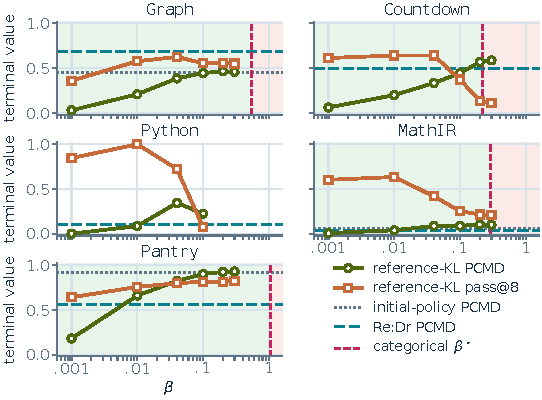
\includegraphics[width=\linewidth]{figures/reference_kl_knee.pdf}
  \caption{\textbf{What a coefficient buys, and where it starts spending.}
  Green is where Proposition~\ref{prop:kl-stationary} still holds stationary
  correctness above one half, red the range past $\beta^\ast$; the damage
  follows that boundary in all four domains carrying one. Python has neither,
  solving too little when frozen to define them.}
  \label{fig:reference-kl-knee}
\end{wrapfigure}

The results above are statements about a flow. This subsection reads them
against measured cells, and the reading changes the conclusion in one place and
sharpens it in two others. Table~\ref{tab:reference-kl-measured} reports
terminal \pmd{} for Dr.GRPO with the same update and fresh-rollout budgets
and a reference KL at
\MDklBetaCount{} coefficients, \MDklBetaList{}, across \MDklDomains{} domains
at Qwen2.5-0.5B and Level~1, beside the matched control and verified-replay
arms. Every cell is the control configuration with $\beta$ alone moved.

\begin{table}[t]
  \centering
  \caption{\textbf{Terminal \pmd{} beside categorical reference values.}
  Columns 11--13 give the frozen reference's conditional diversity and
  the replay occupancy summaries $1-1/\E|\mathcal B|$.
  The former is the interior stationary value in
  Proposition~\ref{prop:kl-stationary}, not a transient upper bound.
  The latter is a Jensen upper bound on the mean uniform-bank limit
  $\E[1-1/|\mathcal B|]$ for nonempty fixed categorical banks; it does not
  certify held-out neural diversity. Re:Dr and Re:Max have separate summaries
  because their discovered banks differ. Every
  column but the $\beta$ ones is the 32-disjoint-stream resample; the $\beta$
  columns use the same estimator on their own disjoint draws. Dashes are
  coefficients a domain does not yet carry, and a superscript on a $\beta$ cell
  is a seed count below the five every other column holds, so a value resting
  on one run is marked where it is read rather than in a note. The last column
  is $\beta^\star=c_G/(-\operatorname{logit}\mu(\mathcal C))$, the coefficient
  at which Proposition~\ref{prop:kl-stationary} puts stationary correctness at
  one half, computed from each domain's own frozen correctness.}
  \label{tab:reference-kl-measured}
  \scriptsize
  \setlength{\tabcolsep}{2.9pt}
  \begin{tabular}{@{}lrrrrrrrrrrrrr@{}}
    \toprule
    & \multicolumn{2}{c}{\textbf{no retention}}
      & \multicolumn{5}{c}{\textbf{$+$ reference KL, by $\beta$}}
      & \multicolumn{2}{c}{\textbf{$+$ memory}}
      & \multicolumn{3}{c}{\textbf{reference values}} & \\
    \cmidrule(lr){2-3}\cmidrule(lr){4-8}\cmidrule(lr){9-10}\cmidrule(lr){11-13}
    \textbf{Domain} & Dr.GRPO & MaxRL
      & $.001$ & $.01$ & $.04$ & $.1$ & $.2$
      & \textbf{Re:Dr} & \textbf{Re:Max}
      & KL & Re:Dr & Re:Max & $\beta^\star$ \\
    \midrule
    % Generated by ops/build_reference_kl_comparison.py; do not hand edit.
  \texttt{Graph}  &  0.003  &  0.148  &  0.029  &  0.207  &  0.385  &  0.444  &  0.465  &  0.458  &  0.686  &  0.625  &  0.45  &  0.75  &  0.70  &  0.55 \\
  \texttt{Countdown}  &  0.004  &  0.022  &  0.060  &  0.198  &  0.333  &  0.444  &  0.568  &  0.587  &  0.497  &  0.531  &  ---  &  0.56  &  0.52  &  0.22 \\
  \texttt{Python}  &  0.000  &  0.000  &  0.000  &  0.086  &  0.344  &  0.225$^{3}$  &  ---  &  ---  &  0.099  &  0.239  &  ---  &  0.15  &  0.42  &  --- \\
  \texttt{MathIR}  &  0.003  &  0.008  &  0.007  &  0.038  &  0.086  &  0.088  &  0.103  &  0.099  &  0.039  &  0.018  &  0.06  &  0.15  &  0.12  &  0.29 \\
  \texttt{Pantry}  &  0.000  &  0.000  &  0.180  &  0.660  &  0.824  &  0.901  &  0.925  &  0.931  &  0.557  &  0.556  &  0.91  &  0.85  &  0.85  &  1.05 \\
  \bottomrule

  \end{tabular}
\end{table}
\paragraph{What the flow got right.}
The observed concentration is consistent with the categorical mechanism
in Corollary~\ref{cor:class-collapse}, although neural training does not
satisfy that corollary's update assumptions. The
control with the same update and fresh-rollout budgets reaches \pmd{} at or below $.004$ in every domain in
the table: not reduced diversity but effectively none, which is what a
winner-take-all limit predicts and what no reweighting of binary outcomes was
able to avoid.

\paragraph{Measured checkpoints differ from the stationary predictions.}
Proposition~\ref{prop:kl-stationary} makes the stationary conditional
$\beta$-free. The measured coefficients order \pmd{} monotonically instead, and
the ordering is stable across seeds. The same proposition puts stationary
correctness at essentially one for every coefficient at or below $.1$, even at
the cohort's narrowest reference ($\mu(\mathcal C)=\MDklMuLow{}$, measured on
the frozen model in \MDklMuLowDomain{}); the $\beta=.1$ cells instead sit near
$\mu(\mathcal C)$ itself rather than near that limit.

These discrepancies show that the stationary categorical predictions do
not quantitatively describe the measured checkpoints. Finite training,
shared parameters, and the sampled adaptive optimizer are all possible
sources of the difference; this comparison does not identify their separate
effects. The boundary-force identities and the two-mode
$\Theta(1/[s\log(1/s)])$ versus $\Theta(\log(1/s))$ recovery comparison
motivate mechanism checks, rather than certify the measured neural rates.

\paragraph{Reference diversity and bank occupancy.}
The table compares quantities with different meanings. For a nonempty fixed
uniform categorical bank of size $k$, the limiting diversity is $1-1/k$.
Across such banks, its mean is $\E[1-1/k]\le1-1/\E[k]$ by Jensen's
inequality. The occupancy columns report the latter summary. They are not
exact mean limits when bank sizes differ, and training-bank occupancy does
not furnish a bound on held-out neural PCMD.
The KL column reports the reference conditional, which is the analyzed
interior stationary value rather than a bound on transient diversity.

The measurements nevertheless motivate an occupancy explanation: where
replay discovers few keys, it has few distinct targets to rehearse.
Where the frozen model is broader, KL can preserve useful diversity without
requiring further admission. These are interpretations of the observed
comparison; the categorical results do not identify which mechanism
causes a particular neural outcome.

\paragraph{The fresh objective moves the bound, not just the rate.}
Re:Dr and Re:Max carry separate occupancy columns because a bank is filled by
discovery, and Corollary~\ref{cor:maxrl-starvation} gives MaxRL a coefficient
approaching the group size exactly where correctness is scarce. If that
advantage is real outside the flow it should show up as a fuller bank in the
domain with the least correctness to begin with, and not elsewhere.

That is what the occupancy columns do. In Python, the domain whose control
reaches the lowest correctness of the five, the Re:Max bank holds $1.73$ keys
per prompt against Re:Dr's $1.18$, lifting the occupancy summary from $.15$ to
$.42$ and terminal \pmd{} from $.099$ to $.239$. In the four domains that do
not start starved, the two occupancies differ by at most $.6$ of a key and the
terminal values track them: Re:Max is ahead in Countdown, level in Pantry, and
behind in Graph and MathIR, where its bank is the slightly emptier one. The
prediction was specific --- a discovery advantage confined to small $P$ --- and
the one domain it picks out is the one where it appears.

These measurements are consistent with separating fresh learning and
memory. The per-prompt mean-direction identity does not itself predict the
shared neural trajectory: MaxRL alone reaches $.148$ PCMD in Graph and at
or below $.022$ elsewhere, no better than Dr.GRPO alone in four domains.
The larger Python bank motivates the discovery interpretation, but does not
isolate it from prompt weighting, stochasticity, or optimizer effects.

\paragraph{Consequences for the comparison.}
The claim that a reference KL is the wrong instrument for diversity does not
survive this table and is withdrawn. What survives is narrower and better
specified. Reference KL retains what its reference had; verified replay
rehearses what its bank holds; neither control retains anything. Which of the
first two reaches further is a property of the domain --- the frozen model's
diversity against the bank's realized occupancy --- and not a property of the
method. Sorting the domains by what the best coefficient buys gives three
cases rather than a ranking. In \MDklFreeNames{} an anchor carries more diversity than
either memory arm at no cost in \texttt{pass@8}. In \MDklPricedNames{} it
passes them on diversity only at a coefficient that gives correctness up, which
is a different claim and is read as one below. In \MDklMemoryNames{} no
coefficient reaches either memory arm at all.

The bank-capacity premise of Corollary~\ref{cor:replay-no-collapse}
helps interpret these differences. Lower replay diversity in domains whose
banks remain small is consistent with limited discovery, but occupancy alone
does not separate discovery from retention or bound held-out neural
\pmd{}. The coefficient sweep measures a correctness--diversity tradeoff
at finite checkpoints; it does not establish that the policies reached
their stationary targets. The replay dose also controls restoration time
in Theorem~\ref{thm:replay-finite-recovery}. A matched replay-dose sweep
would be needed to compare those sensitivities empirically.

\subsection{Why a memory rather than an anchor, once the reference is collapsed}
\label{app:theory-kl-case}

App.~\ref{app:theory-kl-measured} withdrew the claim that a reference KL is the
wrong instrument for diversity, because in \MDklFreeDomains{} of \MDklDomains{}
domains it reaches further than either memory arm and gives up no correctness
doing it. This subsection states what remains of the
case for a memory, and it is not a restatement of the withdrawn claim. The
argument is about which of the two quantities a practitioner is relying on, and
about what that quantity is worth in the setting this paper measures.

\paragraph{The case for the anchor, at its strongest.}
For every $\beta>0$, the analyzed reference-KL flow has a full-support
stationary point. It needs no replay bank, admission rule, or bank capacity,
although it retains a reference policy, and adds a familiar loss term. Its best cell is \MDklWinDomain{} at $\beta=\MDklWinBeta{}$,
where it reaches $\pmd{}=\MDklWinPmd{}$ against the better memory arm's
$\MDklWinRivalPmd{}$ with \texttt{pass@8} of $\MDklWinPass{}$ against
$\MDklWinRivalPass{}$: more diversity and no less correctness. That cell rests on
\MDklWinSeeds{} of the five seeds its column will carry, which is why the table
marks it, but nothing in this appendix disputes the measurement, and a reader
choosing a method for a domain that resembles \MDklWinDomain{} should choose
the anchor.

\paragraph{What the anchor is actually buying.}
Proposition~\ref{prop:kl-stationary} says the quantity being bought is the
reference's own success-conditional diversity, and
App.~\ref{app:theory-kl-measured} finds the measured arms at $91$ to $100$
percent of it. This empirical agreement is consistent with reference
retention, while the stationary formula alone does not describe the finite
training trajectory or establish a bound on its diversity.

This is why \MDklWinDomain{} is the case it is. The frozen Qwen2.5-0.5B has
$\pmd{}=\MDklWinFrozenPmd{}$ there, and $.85$ is the most a capacity-16 bank assembles from
$18.19$ admissible keys per prompt. The anchor wins because the reference is
broader than anything the bank can hold --- not because copying is a better
mechanism than accumulating, but because in that one cell there is more worth
copying than the bank can accumulate.

\paragraph{How often is there that much worth copying?}
This paper measures the answer for deployed models.
Section~\ref{sec:hosted-concentration} reports \MDklHostedModels{} hosted
deployments across the benchmark; their macro \pmd{} spans
\MDklHostedRange{}, with \MDklHostedHiModel{} highest at \MDklHostedHi{}. Of
the \MDklHostedCells{} reportable model--domain--level cells in that cohort,
\MDklHostedCellsHalf{} reach $\pmd{}=.50$ and the highest of any of them is
\MDklHostedCellMax{}. \MDklTopFrozenDomain{}'s frozen \MDklTopFrozenPmd{} is
not a typical reference; it is higher than every cell of every frontier model
we measured, including their own \MDklTopFrozenDomain{} cells.

Under Proposition~\ref{prop:kl-stationary}, a deployed model used as the
reference would determine the categorical stationary conditional. Its
measured diversity therefore describes a candidate target; it is not a
ceiling on a retrained neural policy. The
\MDklTopMemoryArm{} result of \MDklTopMemoryPmd{} in
\MDklTopMemoryDomain{} concerns a different evaluation population from
the hosted macro average. The structural distinction is the source of the
target: verified replay uses discovered bank membership, whereas the
analyzed reference-KL target uses the fixed reference distribution.

\paragraph{Three further asymmetries, in decreasing strength.}
The measured knee is the sharpest. In \MDklPricedNames{} every coefficient
that carries the anchor past the memory arms on diversity also costs correctness,
and the steepest of them is \MDklKneeDomain{} at $\beta=\MDklKneeBeta{}$, where
\pmd{} reaches $\MDklKneePmd{}$ against $\MDklKneeRivalPmd{}$ while
\texttt{pass@8} falls to $\MDklKneePass{}$ from $\MDklKneeRivalPass{}$. The
diversity is real and so is the price; in those domains no coefficient buys the
first without the second.

The coefficient is also domain-dependent in a way the dose is not, and the
table's last column says why: $\beta^\star$, the coefficient at which
Proposition~\ref{prop:kl-stationary} halves stationary correctness, is set by
each domain's own frozen correctness and runs from $\MDklBetaStarLo{}$ to
$\MDklBetaStarHi{}$ across the domains that carry one. A practitioner must therefore locate a window whose position
depends on the reference's correctness, the group size and the estimator, per
domain, before training. Replay has the same categorical limit for every positive dose, but its
finite-time restoration still depends on the dose relative to fresh
concentration pressure.

Last and most structural: an anchor requires a reference that is worth
anchoring to, and successive rounds of RL do not supply one. The bank is
assembled from the policy's own verified successes and is available on the
second round for the same reason it was on the first.

\paragraph{What would change this reading.}
The argument rests on a measured claim about references, not a theorem about
mechanisms, so it is defeasible in an obvious way: a setting whose base
policies carry diversity like \MDklWinDomain{}'s, rather than like the hosted
cohort's, is a setting where anchoring is the better primitive and this
appendix says so.
The evidence here is also thin exactly where it is most favourable to the
anchor. \MDklThinCells{} of the \MDklTotalCells{} measured coefficient cells
stand on fewer than five seeds and the thinnest on \MDklSeedsMin{}, the table
marks each one, and the cells still filling are the high-$\beta$ ones the
anchor's case rests on. MathIR's support is keyed to derivations rather than to
answers besides, so a mode certified there need not be one any policy produces.
The anchor's free wins are also the domains where the bank is furthest from
holding what the prompt admits, which is the reading
App.~\ref{app:theory-kl-measured} already gives them: they are discovery
failures on the memory side rather than retention successes on the anchor's.
One of them does not even fit the inheritance account, since a reference that
verifies nothing has no success-conditional diversity to pass on, so what the
coefficient supplies there cannot be inferred from the stationary
conditional formula. Zero observed successes also does not establish
zero population correctness. We report them as wins regardless.

\subsection{Scope relative to entropy, KL, admission, and neural optimization}
\label{app:theory-entropy}
\label{app:theory-entropy-comparison}

\paragraph{Dependence on optimization geometry.}
For a smooth parameterization $z=z(\theta)$ with Jacobian
$J_\theta=\partial z/\partial\theta$, Euclidean parameter flow instead
induces $\dot z=c_G(P)J_\theta J_\theta^\top\nabla_zP$. The independently
trained logit theorem uses $J_\theta J_\theta^\top=I$ and does not automatically
extend to arbitrary shared parameters or another optimization metric. Equal
binary reward alone does not force this winner selection. The natural policy
gradient update of \citet[Lemma~15]{agarwal2021policygradient}, specialized to
this bandit, is $p_a^+\propto p_a\exp(\eta c_G(P)R_a)$ and preserves
every ratio of correct probabilities at each finite step. Its continuous
version has $\dot z_a=c_G(P)(R_a-P)$, with
$R_a=\1[a\in\mathcal C]$. The distinction between Euclidean and natural
updates also underlies the tabular entropy identities of
\citet[Theorems~1--2]{cui2025entropy}; entropy and verified-mode diversity
remain different observables.

The mean-gradient identity has broader scope than the collapse conclusion.
For one prompt and a common autonomous preconditioner $M(\theta)$, positive
coefficients give flows $c_a(P)M(\theta)\nabla_\theta P$ that follow the same
orbit after a change of time. Outcome-dependent covariance, response-length
weights, shared prompts, and optimizer memory can break the corresponding
training-trajectory equivalence, as the preceding neural analysis shows.
Parameter count alone does not identify this geometry. The empirical scale
comparisons change pretrained models and schedules; they do not establish
the cause of cross-scale differences or the training history of a hosted
model.

A bounded advantage based on fresh samples has a different boundary behavior.
The next bound includes group-dependent detached scores and distinguishes
sampled updates from gradients of an exactly evaluated entropy functional.

\begin{lemma}[Bounded sampled scores have no probability-independent boundary force]
\enforcehalffinalproseline
\label{lem:sampled-score-bound}
Under Assumption~\ref{ass:categorical-mean-flow}, condition on the training history, draw
$Z_1,\ldots,Z_G$ independently from $p$, and let $a_i$ be any detached,
possibly group-dependent advantages with $|a_i|\le B$. To interpret the
bound uniformly as $p_b\to0$, assume a finite $B$ independent of that limit.
At the on-policy point define
\[
 \widehat g=\frac1G\sum_{i=1}^G a_i(\mathbf e_{Z_i}-p).
\]
For every category $b$,
\[
 |\E[\widehat g_b]|\le\E|\widehat g_b|
 \le 2B p_b(1-p_b).
\]
On a group with no draw of $b$, exactly
$\widehat g_b=-p_bG^{-1}\sum_i a_i$; it is zero if the applied advantages
sum to zero. By comparison, the verified-replay component for a fixed target
$w$ has logit velocity $\rho(w_b-p_b)$, which approaches $\rho w_b>0$
for a banked category as $p_b\to0$.
\end{lemma}

\begin{proof}
\enforcehalffinalproseline
Use the triangle inequality and $|a_i|\le B$. Each marginal draw satisfies
$\E|\1\{Z_i=b\}-p_b|=2p_b(1-p_b)$, irrespective of the dependence of
$a_i$ on the group. On the absence event all indicator terms are zero.
The replay formula follows by differentiating $-\sum_b w_b\log p_b$.
\end{proof}

The bound compares the isolated logit-gradient components. It does not prove
inevitable collapse, rule out retention by a bounded estimator, or guarantee
that replay dominates the full update. An unsampled mode can still change
through softmax normalization or shared parameters. Exact entropy is outside
the uniformly bounded-score premise because its surprisal is unbounded near
zero; the lemma is not an impossibility result for entropy regularization.
Nor does the absence of a mode from a finite sample establish zero probability.

\paragraph{Exact entropy is a different comparator.}
For a known full correct support and uniform $u$, the elementary identities
\[
 H(q)=\log m-\mathrm{KL}(q\|u),\qquad
 R_u(p)=\log m-\log P+\mathrm{KL}(u\|q)
\]
show that exact conditional entropy and categorical replay both favor a
uniform conditional target. With strictly increasing correctness potential
$\Psi$, both $\Psi(P)+\beta H(q)$ and $\Psi(P)-\rho R_u(p)$ have the unique
global optimum $P=1,q=u$ in probability space on the simplex with $P>0$,
for positive coefficients. This is a boundary limit for finite-logit softmax
policies. The optimum follows from nonnegativity of KL and increasing
$\Psi$; it does not assert convergence of either neural update. The KL direction distinguishes their
loss level sets \citep{pereyra2017confidencepenalty,agarwal2021policygradient}:
replay loss diverges when a protected coordinate vanishes, whereas
conditional entropy can remain $\log(m-1)$ with one missing mode.

Exact full-output entropy is a third objective and also regularizes incorrect
mass. Exact tabular entropy-regularized policy gradient has its own positive
probability and convergence guarantees under specified assumptions
\citep{mei2020softmaxpg}; our collapse theorem contains no entropy term.
The sampled semantic scores in the experiments are not exact gradients of
full-output or conditional verified-key entropy. Neither their empirical
comparison nor the bounded-score lemma is an impossibility result for entropy.

\paragraph{Discovery and optimization remain separate requirements.}
Retention starts after a verified key enters active memory. Actual insertion
depends on generation, validation, capacity, and eligibility; a positive
sampling probability alone does not establish eventual admission. Once a
non-evicting capacity-16 bank fills, an unbanked key can remain ineligible.
Changing membership or exemplar weights changes the loss being bounded, so
fixed-bank descent cannot simply be carried across those changes. In
particular, the fixed-weight argument does not cover a target whose weights
continue to change with fresh observation counts.

For a fixed joint potential, a discrete bound
$F(\theta_{n+1})\le F(\theta_n)+\epsilon_n$ with
$\epsilon_n\ge0$ and $\sum_{n\ge n_0}\epsilon_n=E<\infty$ would extend
Lemma~\ref{lem:shared-exemplar-retention}, using
$D=F(\theta_{n_0})+J_{\max}+E$ for steps $n\ge n_0$.
This follows by telescoping and bounds retention, not convergence. Corollary~\ref{cor:replay-stochastic-energy-budget} instead permits
conditional expected drift with a controlled accumulated error budget,
and yields a simultaneous probability statement over iterations and
protected exemplars. An optimizer-specific argument is still needed to
establish either form of energy control. A positive replay coefficient or small nominal
learning rate does not establish it. Adam moments, clipping, momentum, prompt
scheduling, and bank changes are not covered by the exact-flow proofs.
The experiments have not established the required joint-energy or
update-error assumptions. The mathematical contribution is the stated
categorical mechanism and conditional exemplar argument; empirical support
and longitudinal exemplar scores remain separate measurements.

% Shared scientific provenance; operational inventories remain in the repository.

